% Biên dịch bằng LuaLaTeX (đã đặt sẵn trong latexmkrc)
\documentclass[11pt,a4paper]{report}

% ---------- Tiếng Việt + font ----------
\usepackage{fontspec}
\usepackage[vietnamese,provide=*]{babel}
\setmainfont{Noto Serif}
\setsansfont{Noto Sans}
\setmonofont{Noto Sans Mono}[Scale=0.9]

% ---------- Bố cục ----------
\usepackage[margin=2.5cm]{geometry}
\usepackage[parfill]{parskip}        % tách đoạn bằng một dòng trống, không thụt đầu dòng
\usepackage{setspace}
\setstretch{1.25}                    % độ cách dòng của nội dung
\setlength{\emergencystretch}{3em}     % tránh tràn lề với thuật ngữ tiếng Anh dài
\usepackage{titlesec}
\titleformat{\chapter}[hang]{\huge\bfseries\sffamily\color{accent}\raggedright}{\chaptertitlename~\thechapter:}{0.5em}{}
\usepackage{titletoc}
\titlecontents{chapter}[0pt]{\addvspace{0.8em}\bfseries\color{accent}}{\chaptertitlename~\thecontentslabel:\ }{}{\titlerule*[0.6em]{.}\contentspage}
\titleformat{\section}{\Large\bfseries\sffamily\color{accent}}{\thesection}{0.6em}{}
\titleformat{\subsection}{\large\bfseries\sffamily}{\thesubsection}{0.6em}{}
\titleformat{\subsubsection}{\normalsize\bfseries\sffamily}{\thesubsubsection}{0.6em}{}

% ---------- Thành phần thường dùng ----------
\usepackage{amsmath,amssymb}
\usepackage{graphicx}
\graphicspath{{images/}{images/shared/}{images/approaches/}}             % ảnh để trong thư mục images/
\setcounter{tocdepth}{1}
\usepackage{float}                   % [H] = đặt ảnh/bảng đúng chỗ
\usepackage{booktabs,tabularx}
\usepackage{enumitem}
\setlist{nosep, leftmargin=*}
\newlist{checklist}{itemize}{2}
\setlist[checklist]{label=$\square$}
\usepackage{xcolor}
\usepackage{array}
\usepackage{tikz}
\usetikzlibrary{arrows.meta}
\definecolor{accent}{HTML}{1F4E79}
\usepackage[most]{tcolorbox}
\usepackage[numbers]{natbib}
\usepackage[colorlinks=true,linkcolor=accent,citecolor=accent,urlcolor=accent]{hyperref}

% ---------- Khung code ----------
\usepackage{listings}
\definecolor{codebg}{HTML}{F6F8FA}
\lstset{
  basicstyle=\ttfamily\small,
  backgroundcolor=\color{codebg},
  frame=single, rulecolor=\color{black!15},
  numbers=left, numberstyle=\tiny\color{black!45},
  keywordstyle=\color{accent}\bfseries,
  commentstyle=\color{black!55}\itshape,
  stringstyle=\color{red!60!black},
  breaklines=true, showstringspaces=false,
  tabsize=4, columns=fullflexible, keepspaces=true,
  xleftmargin=1.5em, framexleftmargin=1.5em,
}

% ---------- Hộp ghi chú ----------
\newtcolorbox{keyidea}[1][Ý chính]{colback=blue!4, colframe=accent, fonttitle=\bfseries\sffamily, title=#1}
\newtcolorbox{question}[1][Câu hỏi]{colback=orange!5, colframe=orange!70!black, fonttitle=\bfseries\sffamily, title=#1}
\newtcolorbox{warning}[1][Lưu ý]{colback=red!4, colframe=red!60!black, fonttitle=\bfseries\sffamily, title=#1}

\newcommand{\todo}[1]{\textcolor{red}{[TODO: #1]}}


% ---------- Tiêu đề ----------
\title{\sffamily\bfseries Reconstructing Real-World Driving Scenes using NeRF or 3D Gaussian Splatting\\[0.5em]
  \large\mdseries Reference Architecture \& Research Engineering Design}
\author{Lâm Quang Anh Quân \\ Lương Sỹ Khánh \\ Đặng Thái Anh \\ Phạm Minh Hiếu}
\date{\today}

\begin{document}
\maketitle
\tableofcontents

% ---------- Part I: cả nhóm đọc và thống nhất ----------
\part{Shared Foundation}
\chapter{Introduction \& Requirements (Bài toán và yêu cầu)}

\section{Cách dùng tài liệu này}

Tài liệu này có hai vai trò. Trước hết, nó là nền tảng chung để cả nhóm hiểu bài toán theo cùng một cách. Sau đó, nó trở thành nơi ghi lại thực nghiệm của từng thành viên và kết quả tổng hợp của cả nhóm. Ba phần của tài liệu tương ứng với ba phase của project:

\begin{itemize}
  \item \textbf{Part I} được cả nhóm đọc và thống nhất trong Phase 1. Phần này mô tả bài toán, kiến trúc hệ thống, thiết kế framework, protocol đánh giá và kế hoạch nghiên cứu.
  \item \textbf{Part II} được viết trong Phase 2. Mỗi thành viên hoàn thành chương về approach mình phụ trách theo cùng một mẫu, để các chương có thể so sánh trực tiếp với nhau.
  \item \textbf{Part III} được cả nhóm viết trong Phase 3, khi các kết quả của Part II được tổng hợp, so sánh và tích hợp thành pipeline cuối cùng.
\end{itemize}

Vì Part II và Part III đều dựa trên những gì đã thống nhất ở Part I, mỗi thành viên cần tự trả lời được các câu hỏi sau trước khi bắt đầu Phase 2:

\begin{itemize}
  \item Nhóm đang giải quyết bài toán gì?
  \item Hệ thống cuối cùng được kỳ vọng hoạt động như thế nào?
  \item Approach mình được giao đóng vai trò gì trong hệ thống đó?
  \item Mình cần thực nghiệm những gì?
  \item Mình cần cung cấp kết quả và artifact nào để tích hợp vào framework?
\end{itemize}

\section{Goal (Mục tiêu)}

Mục tiêu của project được phát biểu như sau:

\begin{quote}
  \itshape
  Explore existing methods in the field of 3D scene reconstruction
  in order to construct \& develop a scalable, cost-efficient, and reproducible Real-to-Sim pipeline
  that reconstructs real-world road environments
  and enables closed-loop traffic simulation in CARLA.
\end{quote}

Nói cách khác, nhóm cần tìm hiểu các phương pháp tái dựng cảnh 3D hiện có, rồi dựa trên đó xây dựng một pipeline Real-to-Sim, tức là quy trình đi từ dữ liệu ghi lại ở thế giới thực đến một môi trường mô phỏng. Pipeline này phải phục dựng được môi trường giao thông thực tế và cho phép chạy mô phỏng vòng kín (closed-loop) trong CARLA. Ba tính chất được đặt ra cho pipeline là linh hoạt khi mở rộng (scalable), tiết kiệm chi phí (cost-efficient) và chạy lại được với kết quả như cũ (reproducible).

Bên cạnh pipeline, project cần xây dựng một tool hoàn chỉnh để thử nghiệm pipeline của nhiều approach khác nhau. Lý do là các approach không chỉ khác nhau ở thuật toán trong từng bước mà còn có thể khác nhau ở thứ tự các bước. Vì vậy, tool phải cho phép hai việc:

\begin{itemize}
  \item Thay method xử lý trong từng module của pipeline.
  \item Sắp xếp lại thứ tự các module cho phù hợp với từng approach.
\end{itemize}

Với thời lượng 6 tuần, kết quả có giá trị nhất không nhất thiết là scene đẹp nhất. Điều quan trọng hơn là chứng minh được phương pháp nào tái dựng được dữ liệu pinhole/fisheye + LiDAR của nhóm, kèm theo các con số đo được và kiểm chứng được về chất lượng, chi phí và khả năng tích hợp vào mô phỏng.

\section{Requirement specification (Đặc tả yêu cầu)}

Các yêu cầu dưới đây được sắp theo đường đi của dữ liệu qua hệ thống: bắt đầu từ dữ liệu đầu vào, qua việc khảo sát phương pháp và công cụ thử nghiệm, đến kết quả tái dựng và môi trường mô phỏng. Cuối danh sách là các tiêu chí dùng để đánh giá pipeline, sản phẩm báo cáo và các yêu cầu không bắt buộc.

\begin{enumerate}
  \item \textbf{Dữ liệu đầu vào:}
  \begin{itemize}
    \item Nguồn dữ liệu là video từ camera pinhole hoặc fisheye, đi kèm LiDAR.
    \item Hệ thống phải xử lý được cả trường hợp tối thiểu: chỉ có video hoặc ảnh, có thể có hoặc không có LiDAR, và không có sẵn calibration, pose, GPS hay nhãn.
  \end{itemize}
  \item \textbf{Khảo sát phương pháp:}
  \begin{itemize}
    \item Khảo sát các promising approach phù hợp với từng loại dữ liệu nguồn và thực hiện evaluation cho các approach đó.
  \end{itemize}
  \item \textbf{Tool thử nghiệm pipeline:}
  \begin{itemize}
    \item Xây dựng một tool hoàn chỉnh để chạy thử pipeline của các approach khác nhau.
    \item Tool cho phép thay method xử lý trong từng module của pipeline.
    \item Tool cho phép thay đổi thứ tự các module theo từng approach.
  \end{itemize}
  \item \textbf{Kết quả tái dựng:}
  \begin{itemize}
    \item Một reconstruction pipeline hoàn chỉnh cho các promising approach.
    \item Một reconstructed scene dùng làm kết quả demo.
  \end{itemize}
  \item \textbf{Đưa vào mô phỏng CARLA:}
  \begin{itemize}
    \item Thực hiện CARLA integration feasibility study, tức là đánh giá việc đưa scene tái dựng vào CARLA có khả thi hay không và vướng ở đâu.
    \item Road logic layer: biểu diễn được mạng đường, gồm hình dạng đường, làn xe, hướng di chuyển, giao lộ, cách các làn nối với nhau và các quy tắc giao thông cơ bản.
    \item Traffic simulation: có các phương tiện khác di chuyển và tương tác với ego vehicle.
    \item Closed-loop simulation trên một khu vực địa lý có thật: xe phải điều khiển được và tương tác được với môi trường được tạo từ một địa điểm thực.
  \end{itemize}
  \item \textbf{Tiêu chí chất lượng của pipeline:}
  \begin{itemize}
    \item Cost efficiency (tiết kiệm chi phí): hạn chế việc dựng map thủ công, quá trình training quá đắt và sự phụ thuộc vào hardware lớn.
    \item Scalability (khả năng mở rộng): pipeline phải tái sử dụng được trên nhiều khu vực, thay vì phải làm thủ công cho từng scene.
    \item Determinism (tính tất định): khi chạy lại cùng một scenario trong cùng điều kiện, pipeline phải cho kết quả nhất quán.
  \end{itemize}
  \item \textbf{Báo cáo:}
  \begin{itemize}
    \item Evaluation \& technical report.
  \end{itemize}
  \item \textbf{Nice to have:}
  \begin{itemize}
    \item Sensor model: mô phỏng camera, LiDAR hoặc các đặc tính khác của cảm biến.
    \item Vehicle modeling: xây dựng mô hình động lực học xe chuyên biệt và chính xác hơn.
  \end{itemize}
\end{enumerate}

\section{Scope (Phạm vi)}

Real2Sim Studio được thiết kế như một framework hoàn chỉnh, gồm các module độc lập, và trong mỗi module các method thuật toán có thể thay thế cho nhau. Kiến trúc tổng thể này không bị giới hạn bởi thời lượng 6 tuần. Trong 6 tuần, nhóm hiện thực hóa và kiểm chứng được phần nào thì tài liệu ghi nhận đúng phần đó.

Do thiết kế rộng hơn những gì kịp làm, một thành phần có thể đang ở các mức hoàn thiện khác nhau. Một module có thể đã được thiết kế nhưng chưa được triển khai, và một module đã triển khai cũng chưa chắc đã được kiểm chứng đầy đủ. Để người đọc không nhầm giữa ``đã thiết kế'' và ``đã chạy đúng'', tài liệu luôn phân biệt ba khái niệm sau:

\begin{table}[H]
  \centering
  \caption{Ba trạng thái của một thành phần}
  \begin{tabularx}{\linewidth}{>{\raggedright\arraybackslash}p{3.6cm} X}
    \toprule
    \textbf{Khái niệm} & \textbf{Ý nghĩa} \\
    \midrule
    1. Reference architecture & Thiết kế của toàn bộ hệ thống lý tưởng: chức năng, module, luồng dữ liệu và interface \\
    \addlinespace
    2. Implementation & Những thành phần nhóm đã thực sự phát triển hoặc tích hợp \\
    \addlinespace
    3. Validation & Những thành phần đã chạy thử và có bằng chứng hoạt động đúng \\
    \bottomrule
  \end{tabularx}
\end{table}

\section{Deliverables}

Bảng dưới đây liệt kê các sản phẩm nhóm sẽ bàn giao khi kết thúc project. Đây mới là bản đề xuất: điều kiện nghiệm thu của từng sản phẩm vẫn cần mentor xác nhận.

\begin{table}[H]
  \centering
  \small
  \caption{Danh sách deliverables}
  \begin{tabularx}{\linewidth}{>{\raggedright\arraybackslash}p{3.3cm} >{\raggedright\arraybackslash}p{3.2cm} l >{\raggedright\arraybackslash}X}
    \toprule
    \textbf{Deliverable} & \textbf{Định dạng} & \textbf{Phụ trách} & \textbf{Điều kiện nghiệm thu} \\
    \midrule
    Tool thử nghiệm pipeline & Mã nguồn và hướng dẫn chạy & TBD & Đổi được method và thứ tự module, chạy lại được \\
    \addlinespace
    Reconstruction pipeline & Mã nguồn và config & TBD & Chạy được từ dữ liệu đến ảnh render \\
    \addlinespace
    Scene demo & Video và file scene & TBD & Render được đoạn đường đã chọn \\
    \addlinespace
    Bảng benchmark & Bảng số liệu và log & TBD & Cùng dataset và cùng protocol ở chương 4 \\
    \addlinespace
    CARLA feasibility study & Một chương trong báo cáo & TBD & Có feasibility matrix và nêu rõ hạn chế \\
    \addlinespace
    Technical report & PDF & TBD & Đủ các chương, được mentor đánh giá \\
    \bottomrule
  \end{tabularx}
\end{table}

\chapter{Real2Sim System Architecture (Kiến trúc hệ thống tham khảo)}

Chương này mô tả một pipeline tổng quát để đạt được các deliverable và giúp cả nhóm nhìn được bức tranh chung của hệ thống, chứ không phải pipeline bắt buộc: mỗi hệ thống hoặc approach thực tế có thể tổ chức các bước theo cách khác và dùng những method khác nhau.

\section{Phương pháp thiết kế}

Nhóm không chọn công nghệ ngay từ đầu.
Trước tiên, nhóm đọc yêu cầu, xác định sản phẩm cần có, chia hệ thống thành các khối chức năng và quy định các khối trao đổi dữ liệu với nhau thế nào.
Sau đó, nhóm mới tìm cách làm cho từng khối và chạy thử.

\begin{figure}[H]
  \centering
  \begin{tikzpicture}[
      box/.style={draw=accent, fill=blue!4, rounded corners=2pt, align=center,
                  minimum width=2.8cm, text width=2.6cm, minimum height=1.1cm,
                  font=\scriptsize\sffamily},
      ask/.style={box, fill=orange!10, draw=orange!70!black},
      flow/.style={-{Stealth[length=2mm]}, thick, color=black!65},
      lbl/.style={font=\scriptsize\sffamily, color=black!70}]
    \node[box] (r) at (0,0) {\textbf{1. Yêu cầu}\\Đề bài và ràng buộc};
    \node[box] (o) at (3.7,0) {\textbf{2. Sản phẩm cần có}\\Demo, số liệu, báo cáo};
    \node[box] (a) at (7.4,0) {\textbf{3. Kiến trúc}\\Các khối chức năng};
    \node[box] (c) at (11.1,0) {\textbf{4. Nối các khối}\\Mỗi khối nhận gì, trả gì};
    \node[box] (s) at (11.1,-2.6) {\textbf{5. Tìm cách làm}\\Paper, repo, dataset};
    \node[box] (e) at (7.4,-2.6) {\textbf{6. Chạy thử}\\Quy mô nhỏ};
    \node[ask] (q) at (3.7,-2.6) {Kết quả có khớp với thiết kế không?};
    \node[box] (i) at (0,-2.6) {\textbf{7. Ghép và đánh giá}\\Báo cáo, kết luận};
    \draw[flow] (r) -- (o);
    \draw[flow] (o) -- (a);
    \draw[flow] (a) -- (c);
    \draw[flow] (c) -- (s);
    \draw[flow] (s) -- (e);
    \draw[flow] (e) -- (q);
    \draw[flow] (q) -- node[lbl, above] {Có} (i);
    \draw[flow] (q.north) -- ++(0,0.6) -| node[lbl, pos=0.25, above] {Không: sửa kiến trúc} (a.south);
  \end{tikzpicture}
  \caption{Các bước thiết kế hệ thống}
\end{figure}

Điểm quan trọng là mũi tên quay lại: kiến trúc ban đầu chỉ là dự đoán, nên nếu chạy thử cho thấy thiết kế không phù hợp thì nhóm quay lại sửa kiến trúc.

Ví dụ, ban đầu nhóm yêu cầu khối render phải xuất được cả ảnh pinhole và fisheye.
Khi chạy thử, nhóm có thể thấy một phương pháp chỉ hỗ trợ pinhole, còn phương pháp khác hỗ trợ fisheye nhưng không nhận LiDAR.
Lúc đó, nhóm sửa thiết kế để mỗi phương pháp khai báo rõ mình làm được gì, thay vì ép tất cả theo cùng một kiểu.

\section{Một số hệ thống Real2Sim hiện có}

Để hiểu bài toán, nhóm xem 3 hệ thống đã có: NVIDIA NuRec\footnote{\url{https://docs.nvidia.com/nurec/basics/how-nurec-works.html}} kết hợp CARLA\footnote{\url{https://carla.readthedocs.io/en/latest/nvidia_nurec/}}, HUGSIM\footnote{\url{https://arxiv.org/abs/2412.01718}} và Cam2Sim\footnote{\url{https://github.com/ast-fortiss-tum/cam2sim}}.
Cả 3 đều đi theo luồng chung dưới đây, nhưng phạm vi và cách làm ở mỗi khâu khác nhau:

\begin{figure}[H]
  \centering
  \begin{tikzpicture}[
      box/.style={draw=accent, fill=blue!4, rounded corners=2pt, align=center,
                  text width=2.5cm, minimum height=0.9cm, font=\small\sffamily},
      flow/.style={-{Stealth[length=2mm]}, thick, color=black!65},
      evalflow/.style={flow, dashed, color=black!45}]
    \node[box] (a) at (0,0) {Dữ liệu thật};
    \node[box] (b) at (3.6,0) {Thế giới tái dựng};
    \node[box] (c) at (7.2,0) {Mô phỏng};
    \node[box] (d) at (11.2,0) {Tác tử lái};
    \node[box, text width=13.7cm] (e) at (5.6,-1.8) {Đánh giá ở nhiều khâu};
    \draw[flow] (a) -- (b);
    \draw[flow] (b) -- (c);
    \draw[flow] ([yshift=2mm]c.east) -- ([yshift=2mm]d.west);
    \draw[flow] ([yshift=-2mm]d.west) -- ([yshift=-2mm]c.east);
    \foreach \n in {a,b,c,d} \draw[evalflow] (\n.south) -- (\n.south |- e.north);
  \end{tikzpicture}
  \caption{Luồng chung của các hệ thống Real2Sim}
\end{figure}

Tuy nhiên, 3 hệ thống này không dùng chung một pipeline.
Không phải hệ thống nào cũng dùng CARLA, và không phải hệ thống nào cũng có một AD Stack đầy đủ. Chương 5 tổng hợp thêm các hệ thống khác.

\begin{table}[H]
  \centering
  \small
  \caption{So sánh 3 hệ thống thực tế}
  \begin{tabularx}{\linewidth}{>{\raggedright\arraybackslash}p{2.2cm} >{\raggedright\arraybackslash}X >{\raggedright\arraybackslash}X >{\raggedright\arraybackslash}X}
    \toprule
    \textbf{Thành phần} & \textbf{NuRec + CARLA} & \textbf{HUGSIM} & \textbf{Cam2Sim} \\
    \midrule
    Dữ liệu & Camera và LiDAR ở format NCore, kèm dữ liệu phụ trợ & Ảnh RGB, dự đoán semantic và tracking; không cần LiDAR để dựng cảnh & Cần camera và pose, LiDAR tùy chọn; trích xuất từ ROS bag \\
    \addlinespace
    Dựng cảnh & Tách nền tĩnh và vật thể động, xuất USDZ & 3DGS, tách mặt đường, nền tĩnh và xe động & COLMAP chạy thủ công, rồi Splatfacto \\
    \addlinespace
    Bản đồ đường & Gói USDZ có thể kèm bản đồ XODR & Multi-plane ground; HD map chỉ có ở nuScenes & Tải OSM, chuyển sang \texttt{map.xodr} bằng \texttt{carla.\allowbreak Osm2Odr} \\
    \addlinespace
    Mô phỏng & NuRec không tự mô phỏng; chạy với AlpaSim hoặc CARLA & Simulator riêng, dùng Gymnasium API & CARLA \\
    \addlinespace
    Xe khác & Có vật thể động, hành vi do simulator quản lý & Replay, IDM, hành vi tấn công & Chỉ có xe đỗ, chưa có traffic động \\
    \addlinespace
    Tạo ảnh cảm biến & gsplat, gọi qua gRPC & Gaussian renderer tích hợp & Splatfacto hoặc camera của CARLA \\
    \addlinespace
    Tác tử lái & Vòng kín qua AlpaSim; ví dụ CARLA dùng bộ bám quỹ đạo, chưa nối AD Stack & UniAD, VAD, Latent-TransFuser & DAVE-2 \\
    \addlinespace
    Đánh giá & Kiểm tra dữ liệu, validation (PSNR), so sánh hình ảnh và hành vi, benchmark & PSNR, SSIM, LPIPS, KID; HD-Score cho lái xe & Semantic IoU; Fréchet distance, tỷ lệ ra khỏi hành lang, steering jitter \\
    \bottomrule
  \end{tabularx}
\end{table}

Có 3 điểm đáng chú ý:
\begin{itemize}
  \item \textbf{NuRec} lo dựng cảnh và render, không tự chạy mô phỏng. Trong luồng với CARLA, CARLA tải bản đồ và các xe, còn NuRec trả ảnh qua gRPC. Tài liệu CARLA gọi ví dụ này là replay, nhưng mã nguồn đã có điểm nhận lệnh lái, chỉ chưa nối AD Stack (xem chương 11). Vòng kín của NuRec được NVIDIA mô tả đầy đủ qua AlpaSim, một simulator mã nguồn mở.
  \item \textbf{HUGSIM} là simulator closed-loop hoàn chỉnh, có runtime riêng, không chạy trên CARLA. Cảnh được dựng từ ảnh RGB, không cần LiDAR.
  \item \textbf{Cam2Sim} là pipeline end-to-end trên CARLA, gồm 6 bước từ trích xuất dữ liệu đến đánh giá. Hệ thống có 4 chế độ chạy: replay trên CARLA, replay bằng Gaussian Splatting, và closed-loop với DAVE-2 trên ảnh CARLA hoặc ảnh Gaussian Splatting. Hiện hệ thống mới có xe đỗ, chưa có traffic động.
\end{itemize}

=> Vì mỗi hệ thống tổ chức khác nhau, điều cần chuẩn hóa không phải là thứ tự các thuật toán, mà là các chức năng hệ thống phải có và cách các chức năng đó trao đổi dữ liệu với nhau.

\section{Tổng quan hệ thống}

Từ nhận xét trên, kiến trúc được định nghĩa theo 5 chức năng, gọi là 5 subsystem, và chia thành 2 giai đoạn:
\begin{itemize}
  \item \textbf{Offline:} xử lý dữ liệu đã ghi để tạo ra thế giới tái dựng.
  \item \textbf{Online:} chạy mô phỏng theo từng bước thời gian, trên thế giới đó.
\end{itemize}

\begin{figure}[H]
  \centering
  \begin{tikzpicture}[
      box/.style={draw=accent, fill=white, rounded corners=2pt, align=center,
                  text width=2.5cm, minimum height=1cm, inner sep=2pt,
                  font=\fontsize{7}{8.5}\selectfont\sffamily},
      head/.style={font=\fontsize{7}{8.5}\selectfont\sffamily\bfseries, color=accent, anchor=north},
      stage/.style={font=\scriptsize\sffamily\bfseries, color=black!60, anchor=north west},
      group/.style={draw=accent, fill=blue!4, rounded corners=3pt},
      flow/.style={-{Stealth[length=2mm]}, thick, color=black!65},
      evalflow/.style={flow, dashed, color=black!45},
      lbl/.style={font=\tiny\sffamily, color=black!70, align=center}]
    \fill[black!3, rounded corners=4pt] (-1.3,-2.75) rectangle (7.0,2.75);
    \fill[black!3, rounded corners=4pt] (7.2,-2.75) rectangle (14.6,2.75);
    \node[stage] at (-1.25,2.72) {OFFLINE: tái dựng thế giới};
    \node[stage] at (7.25,2.72) {ONLINE: mô phỏng closed-loop};
    \node[box, fill=blue!4, text width=2.1cm] (data) at (0,0) {\textbf{1. Data}\\camera, LiDAR, calibration, pose};
    \draw[group] (2.0,-2.45) rectangle (6.7,2.2);
    \node[head] at (4.35,2.15) {2. World Construction};
    \node[box, text width=4.1cm] (visual) at (4.35,1.2) {Cảnh hình ảnh\\3DGS, NeRF, mesh};
    \node[box, text width=4.1cm] (road) at (4.35,-0.1) {Đường và thế giới vật lý\\bản đồ, geometry, semantics};
    \node[box, text width=4.1cm] (actor) at (4.35,-1.4) {Vật thể động\\quỹ đạo, mô hình vật thể};
    \draw[group] (7.6,-1.9) rectangle (10.8,2.2);
    \node[head] at (9.2,2.15) {3. Simulation Runtime};
    \node[box] (sim) at (9.2,1.05) {CARLA hoặc simulator khác};
    \node[box] (sensor) at (9.2,-0.95) {Sensor rendering\\camera, LiDAR};
    \node[box, fill=blue!4, text width=2.1cm] (ad) at (13.2,0) {\textbf{4. AD Stack / Agent}\\perception, planning, control};
    \node[box, fill=blue!4, text width=15.6cm, minimum height=0.75cm] (eval) at (6.65,-3.4) {\textbf{5. Evaluation \& Experiment Framework}};
    \draw[flow] (data.east) -- (2.0,0);
    \draw[flow] (6.7,0) -- (7.6,0);
    \draw[flow] (sim) -- node[lbl, right] {trạng thái\\thế giới, xe} (sensor);
    \draw[flow] (sensor.east) -| node[lbl, below, pos=0.35] {dữ liệu cảm biến} (ad.south);
    \draw[flow] (ad.north) |- node[lbl, above, pos=0.7] {lệnh điều khiển} (sim.east);
    \draw[evalflow] (0,-1) -- (0,-3.02);
    \draw[evalflow] (4.35,-2.45) -- (4.35,-3.02);
    \draw[evalflow] (9.2,-1.9) -- (9.2,-3.02);
    \draw[evalflow] (14.0,-0.8) -- (14.0,-3.02);
  \end{tikzpicture}
  \caption{Reference architecture theo 5 subsystem}
\end{figure}

Đây là kiến trúc do nhóm đề xuất, không phải sơ đồ được công bố nguyên dạng bởi NVIDIA hay một tổ chức tiêu chuẩn.
Sơ đồ mô tả chức năng, không phải một pipeline bắt buộc chạy tuần tự.
Một approach cụ thể có thể gộp nhiều module thành một.

NuRec không phải toàn bộ kiến trúc, mà là một implementation có thể cung cấp một số chức năng trong đó.
Tương tự, 3DGUT là công nghệ có thể dùng bên trong World Construction hoặc rendering.

\section{Subsystem 1: Data}

Subsystem này biến dữ liệu thô ghi từ xe thành một dataset chuẩn, để mọi approach phía sau dùng chung.
Đây là phần đầu của toàn bộ hệ thống: nếu dữ liệu ở đây sai, ví dụ camera và LiDAR bị lệch nhau, thì cảnh dựng ra và kết quả đánh giá phía sau đều sai theo.

\begin{figure}[H]
  \centering
  \begin{tikzpicture}[
      box/.style={draw=accent, fill=blue!4, rounded corners=2pt, align=center,
                  text width=1.72cm, minimum height=1cm, inner sep=1pt,
                  font=\fontsize{6.5}{8}\selectfont\sffamily},
      src/.style={box, fill=blue!12},
      head/.style={font=\fontsize{6.5}{8}\selectfont\sffamily\bfseries, color=accent, align=center, text width=1.9cm},
      lane/.style={font=\scriptsize\sffamily\bfseries, color=black!60, anchor=west},
      flow/.style={-{Stealth[length=2mm]}, thick, color=black!65}]
    \node[head] at (2.1,1.95) {1. Đọc dữ liệu};
    \node[head] at (4.2,1.95) {2. Đồng bộ thời gian};
    \node[head] at (6.3,1.95) {3. Calibration};
    \node[head] at (8.4,1.95) {4. Pose};
    \node[head] at (10.5,1.95) {5. Nhãn vật thể};
    \node[lane] at (-0.86,1.5) {Đường A};
    \node[lane] at (-0.86,-1.65) {Đường B};
    \node[src] (a0) at (0,0.8) {Dataset có sẵn};
    \node[box] (a1) at (2.1,0.8) {Chuyển format};
    \node[box] (a2) at (4.2,0.8) {Dùng thời gian có sẵn};
    \node[box] (a3) at (6.3,0.8) {Dùng calibration có sẵn};
    \node[box] (a4) at (8.4,0.8) {Dùng pose có sẵn};
    \node[box] (a5) at (10.5,0.8) {Dùng nhãn có sẵn};
    \node[src] (b0) at (0,-0.8) {Log thô: video hoặc ảnh, có thể có LiDAR};
    \node[box] (b1) at (2.1,-0.8) {Tách ảnh, giữ thời gian};
    \node[box] (b2) at (4.2,-0.8) {Ghép dữ liệu, ước lượng độ lệch};
    \node[box] (b3) at (6.3,-0.8) {Tự hiệu chuẩn};
    \node[box] (b4) at (8.4,-0.8) {Tính từ LiDAR hoặc ảnh};
    \node[box] (b5) at (10.5,-0.8) {Chạy model tạo nhãn};
    \node[box] (chk) at (12.35,0) {6. Kiểm tra};
    \node[src] (out) at (14.2,0) {7. Dataset chuẩn};
    \foreach \x/\y in {a0/a1,a1/a2,a2/a3,a3/a4,a4/a5,b0/b1,b1/b2,b2/b3,b3/b4,b4/b5} \draw[flow] (\x) -- (\y);
    \draw[flow] (a5) -- (chk);
    \draw[flow] (b5) -- (chk);
    \draw[flow] (chk) -- (out);
    \draw[-{Stealth[length=2mm]}, thick, dashed, color=black!50] (b4.south) -- ++(0,-0.3) -| node[pos=0.25, below, font=\tiny\sffamily, color=black!70] {tinh chỉnh lại} (b2.south);
    \draw[-{Stealth[length=2mm]}, thick, dashed, color=black!50] (8.4,-1.62) -| (b3.south);
  \end{tikzpicture}
  \caption{Luồng xử lý của subsystem Data}
\end{figure}

\subsection{Đầu vào}

Đầy đủ nhất, subsystem dùng các dữ liệu sau:

\begin{table}[H]
  \centering
  \small
  \caption{Dữ liệu đầu vào}
  \begin{tabularx}{\linewidth}{>{\raggedright\arraybackslash}p{2.9cm} >{\raggedright\arraybackslash}X >{\raggedright\arraybackslash}X l}
    \toprule
    \textbf{Dữ liệu} & \textbf{Là gì} & \textbf{Dùng để làm gì} & \textbf{Mức cần} \\
    \midrule
    \multicolumn{4}{l}{\textbf{Dữ liệu cốt lõi}} \\
    Camera pinhole & Chuỗi ảnh theo thời gian, ảnh ít méo & Dựng hình ảnh của cảnh & Cần ít nhất \\
    \addlinespace
    Camera fisheye & Chuỗi ảnh góc rộng, méo mạnh & Dựng hình ảnh, nhìn được rộng hơn & một camera \\
    \addlinespace
    LiDAR & Các đám mây điểm đo khoảng cách & Dựng hình học, có tỉ lệ thật, kiểm tra căn chỉnh & Nên có \\
    \midrule
    \multicolumn{4}{l}{\textbf{Dữ liệu bổ sung}} \\
    Intrinsics & Thông số bên trong camera: tiêu cự, tâm ảnh, độ méo & Biết điểm 3D rơi vào pixel nào & Tự tạo được \\
    \addlinespace
    Extrinsics & Vị trí và hướng lắp từng cảm biến trên xe & Đưa dữ liệu các cảm biến về cùng hệ tọa độ & Tự tạo được \\
    \addlinespace
    Thời gian ghi & Mốc thời gian của từng ảnh và từng lần quét LiDAR & Ghép đúng dữ liệu cùng thời điểm & Tự tạo được \\
    \addlinespace
    Ego pose & Vị trí và hướng của xe theo thời gian & Biết mỗi ảnh được chụp từ đâu & Tự tạo được \\
    \addlinespace
    Nhãn vật thể & Khung 3D và quỹ đạo của xe, người & Tách vật thể động & Tự tạo được \\
    \addlinespace
    Bản đồ & Bản đồ đường của khu vực, nếu có & Hỗ trợ road logic và khớp tọa độ & Tùy chọn \\
    \addlinespace
    GPS, IMU, CAN & Vị trí, gia tốc, tốc độ, góc lái & Tính ego pose, đối chiếu hành vi lái & Tùy chọn \\
    \bottomrule
  \end{tabularx}
\end{table}

Dữ liệu chia thành 2 nhóm. Nhóm cốt lõi là dữ liệu cảm biến, đo trực tiếp từ môi trường và không thể tự tạo ra. Nhóm bổ sung giúp kết quả tốt hơn, nhưng nếu thiếu thì tự tạo từ nhóm cốt lõi hoặc bỏ qua.
Sơ đồ dưới đây cho biết từ các dữ liệu đó tạo ra được gì. Dòng nhỏ trong mỗi ô là dữ liệu cần dùng:

\begin{figure}[H]
  \centering
  \begin{tikzpicture}[
      core/.style={draw=accent, very thick, fill=accent!18, rounded corners=2pt, align=center,
                   text width=2.9cm, minimum height=0.8cm, inner sep=2pt,
                   font=\fontsize{7}{8.5}\selectfont\sffamily\bfseries},
      extra/.style={draw=black!55, dashed, fill=white, rounded corners=2pt, align=center,
                    text width=2.9cm, minimum height=0.56cm, inner sep=1pt,
                    font=\fontsize{7}{8.5}\selectfont\sffamily},
      made/.style={draw=accent, fill=blue!4, rounded corners=2pt, align=center,
                   text width=3.5cm, minimum height=0.92cm, inner sep=2pt,
                   font=\fontsize{7}{8.5}\selectfont\sffamily},
      frame/.style={draw=black!30, rounded corners=4pt, fill=black!2},
      head/.style={font=\scriptsize\sffamily\bfseries, color=accent, anchor=north, align=center},
      flow/.style={-{Stealth[length=2.2mm]}, very thick, color=black!60},
      dflow/.style={flow, dashed, color=black!45},
      lbl/.style={font=\tiny\sffamily, color=black!70, align=center}]
    \fill[black!2, draw=accent, very thick, rounded corners=4pt] (-1.8,1.05) rectangle (1.8,4.5);
    \node[head] at (0,4.43) {Dữ liệu cốt lõi};
    \draw[frame, dashed] (-1.8,-3.6) rectangle (1.8,0.85);
    \node[head, color=black!60] at (0,0.8) {Dữ liệu bổ sung};
    \draw[frame] (3.1,-3.6) rectangle (7.0,4.5);
    \node[head] at (5.05,4.43) {Tự tạo được};
    \draw[frame] (8.3,-3.6) rectangle (12.2,4.5);
    \node[head] at (10.25,4.43) {Thế giới tái dựng};
    \node[core] at (0,3.45) {Camera pinhole};
    \node[core] at (0,2.5) {Camera fisheye};
    \node[core] at (0,1.55) {LiDAR};
    \node[extra] at (0,-0.1) {Calibration};
    \node[extra] at (0,-0.7) {Thời gian ghi};
    \node[extra] at (0,-1.3) {Ego pose, GPS, IMU};
    \node[extra] at (0,-1.9) {CAN: tốc độ, góc lái};
    \node[extra] at (0,-2.5) {Nhãn khung 3D};
    \node[extra] at (0,-3.1) {HD map};
    \node[made] (intr) at (5.05,3.45) {\textbf{Intrinsics}\\camera};
    \node[made] (extr) at (5.05,2.25) {\textbf{Extrinsics}\\camera + LiDAR};
    \node[made] (pose) at (5.05,1.05) {\textbf{Pose, quỹ đạo xe}\\camera hoặc LiDAR};
    \node[made] (scale) at (5.05,-0.15) {\textbf{Tỉ lệ thật (mét)}\\LiDAR, hoặc GPS, tốc độ};
    \node[made] (label) at (5.05,-1.35) {\textbf{Mặt nạ, khung 3D, tracking}\\camera, LiDAR qua model};
    \node[made] (cloud) at (5.05,-2.55) {\textbf{LiDAR gộp nhiều lần quét}\\LiDAR + pose};
    \node[made] (vis) at (10.25,3.2) {\textbf{Cảnh nền 3DGS hoặc NeRF}\\ảnh + calibration + pose + mặt nạ};
    \node[made] (act) at (10.25,1.4) {\textbf{Vật thể động: Gaussian hoặc asset 3D}\\ảnh + pose + khung 3D, tracking};
    \node[made] (geo) at (10.25,-0.4) {\textbf{Hình học vật lý: mặt đường}\\sinh từ map.xodr; mesh là tùy chọn};
    \node[made] (road) at (10.25,-2.2) {\textbf{Road logic: map.xodr}\\OSM, HD map, hoặc quỹ đạo + BEV};
    \draw[flow] (1.8,2.75) -- node[lbl, above] {tính} (3.1,2.75);
    \draw[dflow] (1.8,-1.3) -- node[lbl, above] {dùng ngay\\nếu có} (3.1,-1.3);
    \foreach \a/\b in {intr/vis,extr/vis,pose/vis,label/vis,pose/act,label/act,pose/road}
      \draw[-{Stealth[length=1.6mm]}, color=black!55] (\a.east) -- (\b.west);
    \draw[-{Stealth[length=1.6mm]}, color=black!55] (road.north) -- (geo.south);
    \draw[-{Stealth[length=1.6mm]}, dashed, color=black!55] (cloud.east) -- (geo.west);
    \draw[-{Stealth[length=1.6mm]}, color=black!55] (scale.north) -- (pose.south);
    \draw[-{Stealth[length=1.6mm]}, dashed, color=black!55] (vis.east) -- ++(0.1,0) |- (geo.east);
  \end{tikzpicture}
  \caption{Các loại dữ liệu và những gì tạo ra được từ chúng}
\end{figure}

Một số khái niệm trong sơ đồ:
\begin{itemize}
  \item \textbf{Tỉ lệ thật:} quan hệ giữa kích thước trong mô hình và mét ngoài đời. Chỉ từ một camera thì có hình dạng nhưng không biết độ lớn thật. Tỉ lệ được dùng để đưa pose về đơn vị mét, vì CARLA tính bằng mét.
  \item \textbf{Mặt nạ, khung 3D, tracking:} mặt nạ cho biết pixel nào thuộc vật thể trên ảnh, khung 3D cho biết vị trí và kích thước trong không gian, tracking gán cùng một ID cho vật thể qua các khung hình.
  \item \textbf{LiDAR gộp nhiều lần quét:} mỗi lần quét khá thưa, nên dùng pose đưa các lần quét về cùng hệ tọa độ, sau khi bỏ điểm của xe đang chạy, để có một mô hình 3D dày của con đường.
  \item \textbf{Cảnh nền:} model 3DGS hoặc NeRF của phần tĩnh, dùng để render ảnh.
  \item \textbf{Vật thể động:} có thể là các Gaussian gắn với track, nằm cùng scene với cảnh nền như cách của NuRec, hoặc asset 3D có sẵn do simulator đặt vào.
  \item \textbf{Hình học vật lý:} CARLA sinh mặt đường từ hình dạng và bề rộng đường trong \texttt{map.xodr}, nên không cần xuất mesh. Mesh từ LiDAR hoặc từ cảnh 3DGS (mũi tên nét đứt) là tùy chọn, khi cần nhà và vật cản tĩnh có va chạm.
  \item \textbf{Road logic từ quỹ đạo xe:} xe đã chạy trên đường nên quỹ đạo xấp xỉ một làn đường. Khi không có GPS, hệ thống tạo một con đường dọc theo quỹ đạo, rồi dùng ảnh BEV của mặt đường để bổ sung số làn và bề rộng.
\end{itemize}

Sơ đồ cho thấy vì sao mức tối thiểu vẫn chạy được: chỉ từ camera đã tạo được intrinsics, pose, mặt nạ và khung 3D, rồi đến cảnh hình ảnh và road logic theo quỹ đạo xe.
LiDAR giúp có tỉ lệ thật và hình học chính xác, nên rất nên có. Dữ liệu bổ sung giúp bỏ qua bước tính toán và cho kết quả tốt hơn.

Thực tế có 2 trường hợp, nên hệ thống có 2 đường vào và cùng ra một dataset chuẩn:
\begin{itemize}
  \item \textbf{Đường A, dataset có sẵn:} dataset công khai thường đã có calibration, pose và nhãn khung 3D. Nên dùng luôn, vì nhãn thật thường chính xác hơn nhãn tự tạo. Đường này ít rủi ro và phù hợp để benchmark công bằng.
  \item \textbf{Đường B, chỉ có log thô:} log chỉ gồm video hoặc tập ảnh, có thể có LiDAR. Hệ thống phải tự tạo phần còn thiếu. Đây là mức tối thiểu hệ thống phải hỗ trợ, và cũng đúng với yêu cầu scale up, vì khu vực mới sẽ không có sẵn nhãn.
\end{itemize}

Hai đường không tách hẳn nhau. Nếu dataset chỉ thiếu một phần, ví dụ thiếu nhãn, thì riêng phần đó đi theo cách làm của đường B.
Ở đường B, các mũi tên nét đứt cho biết có thể phải quay lại: sau khi có pose, nhóm dùng pose để bù chuyển động của xe ở bước đồng bộ và tinh chỉnh calibration.

Hệ thống cần xử lý được các mức đầu vào sau. Dữ liệu càng ít thì chất lượng càng giảm, nhưng pipeline vẫn phải chạy được:

\begin{table}[H]
  \centering
  \small
  \caption{Các mức đầu vào hệ thống phải hỗ trợ}
  \begin{tabularx}{\linewidth}{>{\raggedright\arraybackslash}p{3.3cm} >{\raggedright\arraybackslash}X >{\raggedright\arraybackslash}X}
    \toprule
    \textbf{Đầu vào} & \textbf{Hệ thống phải tự tạo} & \textbf{Hạn chế} \\
    \midrule
    Đầy đủ (dataset) & Không cần & Chỉ có ở dataset công khai \\
    \addlinespace
    Video hoặc ảnh + LiDAR & Thời gian, calibration, pose, nhãn & Khó nhất là khớp camera với LiDAR \\
    \addlinespace
    Chỉ có video hoặc ảnh & Intrinsics, pose, tỉ lệ thật, nhãn & Hình học kém hơn, khó biết tỉ lệ thật, không có LiDAR để đánh giá. Một camera trước chỉ thấy một phần cảnh, nên ảnh góc khác kém hơn nhiều \\
    \bottomrule
  \end{tabularx}
\end{table}

Nếu chỉ có LiDAR mà không có ảnh thì dựng được hình học, nhưng không dựng được cảnh hình ảnh, nên đầu vào tối thiểu phải có ảnh.

\subsection{Các bước xử lý}

\textbf{Bước 1: Đọc dữ liệu.}
Mỗi dataset có format riêng, ví dụ ROS bag hoặc thư mục theo cấu trúc của dataset đó, nên cần một bộ chuyển đổi riêng.
Ở bước này cũng kiểm tra nhanh dữ liệu có đủ không, để đổi đoạn khác trước khi tốn thời gian train.
\begin{itemize}
  \item \textbf{Đường A:} chuyển format của dataset về format chung.
  \item \textbf{Đường B:} tách khung hình từ video, ví dụ bằng ffmpeg, và giữ lại thời gian của từng khung. Video và tập ảnh tách sẵn khác nhau không nhiều, nhưng tập ảnh có thể đã mất mốc thời gian gốc, và ảnh từ video thường bị nén nên kém hơn ảnh gốc.
\end{itemize}

\textbf{Bước 2: Đồng bộ thời gian.}
Camera và LiDAR không ghi cùng một lúc, nên phải ghép các dữ liệu có thời điểm gần nhau nhất.
Sai lệch nhỏ cũng gây ảnh hưởng lớn.
Ví dụ, xe chạy 54~km/h (15~m/s), nếu ảnh và LiDAR lệch nhau 50~ms thì xe đã đi được 0,75~m, nên vật thể trong ảnh và trong LiDAR sẽ lệch nhau.
\begin{itemize}
  \item \textbf{Đường A:} dùng mốc thời gian có sẵn và ghép theo thời điểm gần nhất.
  \item \textbf{Đường B:} lấy thời gian từ log của xe. Nếu cảm biến không đồng bộ phần cứng thì phải ước lượng độ lệch. Nếu chỉ có một camera thì không cần ghép, chỉ cần thứ tự khung hình.
\end{itemize}

\textbf{Bước 3: Calibration.}
Calibration cho biết các cảm biến đặt ở đâu so với nhau, và cố định trong suốt quá trình ghi.
Ví dụ, để biết một điểm LiDAR rơi vào pixel nào, trước hết đưa điểm $p_{\text{LiDAR}}$ sang hệ camera bằng phép biến đổi $T$, sau đó chiếu lên ảnh bằng hàm chiếu $\pi$ của camera:
\begin{equation}
  p_{\text{camera}} = T \, p_{\text{LiDAR}}, \qquad \text{pixel} = \pi(p_{\text{camera}})
\end{equation}

Calibration gồm 2 phần: intrinsics cho biết camera chiếu cảnh 3D thành ảnh thế nào, còn extrinsics cho biết cảm biến đặt ở đâu trên xe.
Pinhole và fisheye khác nhau ở hàm chiếu $\pi$. Vì vậy, hai track dùng chung quy trình, chỉ khác mô hình camera.

Khi xe có nhiều camera, kể cả camera có FOV khác nhau, không cần bước riêng.
Mọi cảm biến được quy về cùng một gốc trên xe, gọi là hệ rig. Mỗi camera có một mục riêng trong \texttt{calibration.json}, gồm mô hình camera, intrinsics và extrinsics so với rig.
Ví dụ, xe có 3 camera và 1 LiDAR thì có 3 bộ intrinsics, 4 bộ extrinsics, nhưng chỉ một trajectory của xe.

\begin{itemize}
  \item \textbf{Đường A:} dùng calibration có sẵn, nhưng vẫn kiểm tra lại.
  \item \textbf{Đường B:} intrinsics lấy bằng bảng ô cờ nếu còn tiếp cận được camera (OpenCV), nếu không thì ước lượng từ video (ViPE, COLMAP). Extrinsics giữa camera và LiDAR lấy bằng bảng mục tiêu, hoặc tự động từ cảnh thật. Công cụ direct\_visual\_\allowbreak lidar\_\allowbreak calibration làm được việc này mà không cần bảng mục tiêu, hỗ trợ cả pinhole và fisheye. Nếu không có LiDAR thì không cần phần extrinsics này.
\end{itemize}

\textbf{Bước 4: Pose.}
Pose là vị trí và hướng của xe tại một thời điểm, còn chuỗi pose theo thời gian là trajectory của xe.
Bước này tạo ra trajectory đó. Sau đó, từ pose của xe và calibration, hệ thống suy ra pose của từng camera tại mỗi thời điểm, và đây là thông tin bước dựng cảnh cần.
Đường A dùng pose có sẵn trong dataset, đường B chọn một trong các nguồn còn lại:

\begin{table}[H]
  \centering
  \small
  \caption{Các nguồn pose}
  \begin{tabularx}{\linewidth}{>{\raggedright\arraybackslash}p{3.1cm} >{\raggedright\arraybackslash}X >{\raggedright\arraybackslash}X}
    \toprule
    \textbf{Nguồn} & \textbf{Khi nào dùng} & \textbf{Hạn chế} \\
    \midrule
    Pose có sẵn trong dataset & Dataset đã có và kiểm tra thấy đáng tin & Vẫn phải kiểm tra, không tin tuyệt đối \\
    \addlinespace
    GPS và IMU & Xe có ghi các dữ liệu này & GPS kém chính xác ở khu vực nhiều nhà cao tầng \\
    \addlinespace
    LiDAR odometry & Có LiDAR, cần pose mượt & Sai số tích lũy trên đoạn đường dài \\
    \addlinespace
    ViPE & Chỉ có video. Ước lượng cùng lúc intrinsics, pose và độ sâu gần đúng theo mét, hỗ trợ camera góc rộng & Cần GPU; tỉ lệ chỉ gần đúng, cần kiểm tra trên đường dài \\
    \addlinespace
    Global SfM (SuperPoint, LightGlue) & Chỉ có ảnh, xử lý offline. Dash2Sim dùng hướng này, ghép thêm ảnh Street View để có tỉ lệ thật và vị trí & Cần ảnh tham chiếu ở khu vực đó \\
    \addlinespace
    ORB-SLAM3 & Video liên tục, cần nhanh & Dễ mất dấu khi ít đặc trưng; một camera thì thiếu tỉ lệ thật \\
    \addlinespace
    COLMAP (SfM) & Baseline khi chỉ có ảnh & Chậm, thường kém ổn định với cảnh đường phố; một camera thì thiếu tỉ lệ thật \\
    \bottomrule
  \end{tabularx}
\end{table}

Với LiDAR odometry có thể thử KISS-ICP (chỉ cần LiDAR), hoặc FAST-LIO (cần thêm IMU).
KISS-ICP chỉ tính trajectory của LiDAR, không làm calibration, nên vẫn cần extrinsics từ bước 3 để suy ra pose của camera.

Nếu chỉ dùng một camera, quỹ đạo đúng hình dạng nhưng không biết đơn vị thật. CARLA cần đơn vị mét, nên phải lấy tỉ lệ từ GPS, tốc độ xe, ảnh tham chiếu có vị trí, chiều cao lắp camera, hoặc model ước lượng độ sâu. Trong thử nghiệm của Dash2Sim, model độ sâu một bước chưa đủ chính xác nếu dùng riêng, nên cần kết hợp với hình học nhiều góc nhìn. Tỉ lệ cũng có thể trôi dần trên đoạn đường dài, nên phải kiểm tra lại.
Xe đang chạy trong ảnh cũng có thể làm sai ước lượng, nên cần che các vật thể động trước khi chạy.
Khi có LiDAR thì ưu tiên LiDAR odometry. Khi chỉ có video thì thử ViPE trước, dùng COLMAP làm baseline. Đây là đường tối thiểu hệ thống phải chạy được.

\textbf{Bước 5: Nhãn vật thể.}
Nhãn cho biết xe và người nằm ở đâu, để tách vật thể động khỏi cảnh nền.
\begin{itemize}
  \item \textbf{Đường A:} dùng nhãn khung 3D và quỹ đạo có sẵn.
  \item \textbf{Đường B:} cần 3 việc. Phân đoạn ảnh để có mặt nạ (SegFormer, Mask2Former, SAM). Phát hiện 3D để có khung (PointPillars khi có LiDAR, FCOS3D khi chỉ có ảnh). Tracking để nối khung qua các khung hình, vì hai model phát hiện trên không tự làm việc này. Dash2Sim là ví dụ khi chỉ có ảnh: tracking 2D bằng SAM3, rồi nâng lên 3D nhờ độ sâu, sau đó làm mượt quỹ đạo bằng bộ lọc Kalman. Nhãn tự tạo có thể sai hoặc bỏ sót.
\end{itemize}

Nhãn được lưu riêng trong \texttt{tracks/}, dùng khi train và khi di chuyển vật thể, không phải một phần của ảnh.
Một số hướng giảm phụ thuộc vào nhãn: HUGSIM dùng tracking dự đoán từ model, còn Instant NuRec tự dự đoán quỹ đạo vật thể khi dựng cảnh.

\textbf{Bước 6: Kiểm tra.}
Dù đi theo đường nào, dữ liệu cũng phải qua cùng các kiểm tra trước khi dùng:

\begin{table}[H]
  \centering
  \small
  \caption{Các kiểm tra trên dữ liệu}
  \begin{tabularx}{\linewidth}{>{\raggedright\arraybackslash}p{3.1cm} >{\raggedright\arraybackslash}X >{\raggedright\arraybackslash}X}
    \toprule
    \textbf{Kiểm tra} & \textbf{Cách làm} & \textbf{Nếu bỏ qua} \\
    \midrule
    Đủ dữ liệu & Đếm số ảnh, số lần quét, tìm khung hình thiếu & Pipeline lỗi giữa chừng \\
    \addlinespace
    Thời gian & Kiểm tra thời gian tăng đều, đo độ lệch giữa các cảm biến & Ảnh và LiDAR lệch nhau \\
    \addlinespace
    Calibration & Chiếu LiDAR lên ảnh của từng camera, xem có khớp cạnh vật thể không. Với nhiều camera, xem vùng chồng lấn có khớp không & Cảnh bị mờ, hai nguồn không khớp \\
    \addlinespace
    Pose & Vẽ quỹ đạo, tìm các đoạn nhảy bất thường & Cảnh bị nhòe, đường bị đôi \\
    \addlinespace
    Chất lượng ảnh & Xem nhanh độ mờ, chói, lóa ống kính & Cảnh có vùng lỗi \\
    \bottomrule
  \end{tabularx}
\end{table}

\textbf{Bước 7: Tạo dataset chuẩn.}
Dữ liệu đạt kiểm tra được đưa về một cấu trúc chung, để mọi approach đọc cùng một nguồn. Mỗi approach có một adapter để chuyển từ đây sang format riêng của approach đó.
Cấu trúc dưới đây là đề xuất, sẽ chốt ở chương 3 và chương 4:

\begin{lstlisting}[numbers=none, morecomment={[l]\#}, texcl=true, caption={Cấu trúc dataset chuẩn (đề xuất)}, breaklines=false]
dataset/<sequence>/
  manifest.json       # nguồn dữ liệu, phiên bản, đơn vị, hệ tọa độ
  calibration.json    # intrinsics, extrinsics, loại camera
  poses.csv           # vị trí xe theo thời gian
  images/<camera>/    # ảnh của từng camera
  lidar/              # các lần quét LiDAR
  tracks/             # vật thể động, nếu có
  splits.json         # danh sách ảnh train và ảnh giữ lại để test
\end{lstlisting}

Các công cụ nêu trong mục này là gợi ý, chưa được nhóm chạy thử.

\subsection{Thứ tự làm và rủi ro}

Nên làm đường A trước để benchmark các approach, sau đó thử đường B trên một đoạn ngắn.
Để đo chất lượng đường B, chạy đường này trên chính dataset công khai, rồi so pose và nhãn tự tạo với dữ liệu thật của dataset.

Với đường B khi có LiDAR, mức độ khó theo thứ tự:
\begin{enumerate}
  \item \textbf{Thời gian và extrinsics} rủi ro nhất. Nếu không có thông tin đồng bộ hoặc vị trí lắp cảm biến, camera và LiDAR rất khó khớp, kể cả khi dùng công cụ tự động.
  \item \textbf{Pose} làm được bằng LiDAR odometry, nhưng sai số tích lũy trên đoạn đường dài.
  \item \textbf{Nhãn vật thể} tự tạo được, nhưng cần kiểm tra chất lượng.
\end{enumerate}

Khi chỉ có ảnh, rủi ro lớn nhất chuyển thành tỉ lệ thật và độ ổn định của ước lượng pose. Sai số cũng cộng dồn qua các bước, và các hệ thống hiện có chủ yếu chạy tốt với cảnh ban ngày, thời tiết đẹp.

\subsection{Các module}

\begin{table}[H]
  \centering
  \small
  \caption{Các module của Data}
  \begin{tabularx}{\linewidth}{>{\raggedright\arraybackslash}p{3.6cm} >{\raggedright\arraybackslash}X >{\raggedright\arraybackslash}X}
    \toprule
    \textbf{Module} & \textbf{Làm gì} & \textbf{Không làm gì} \\
    \midrule
    Data ingestion \& standardization & Đọc dữ liệu thô, kiểm tra đủ thành phần, đưa về format chung & Không tính pose, không dựng cảnh \\
    \addlinespace
    Calibration, sync \& localization & Xác định mỗi cảm biến nằm ở đâu, tại thời điểm nào & Không dựng cảnh \\
    \bottomrule
  \end{tabularx}
\end{table}

\subsection{Các hệ thống khác làm thế nào?}

\begin{itemize}
  \item \textbf{NuRec} chuyển dữ liệu sang format chuẩn NCore, kèm một bộ dữ liệu phụ trợ. NVIDIA có công cụ chiếu LiDAR lên ảnh để kiểm tra calibration và thời gian.
  \item \textbf{HUGSIM} dựng cảnh từ ảnh RGB, kèm dự đoán semantic và tracking từ các model có sẵn, nên không cần LiDAR.
  \item \textbf{Cam2Sim} trích xuất dữ liệu từ ROS bag, gồm ảnh, pose đồng bộ theo odometry, LiDAR và góc lái.
\end{itemize}

=> Nhóm cũng cần một format chung như NCore, nhưng không nhất thiết dùng đúng NCore. Mỗi approach có một adapter để chuyển từ dataset chuẩn sang format riêng của approach đó.

\subsection{Việc cần chốt}

\begin{itemize}
  \item Dữ liệu dùng để demo đường B: log của mentor, hay dataset công khai bỏ bớt thông tin?
  \item Dataset cho từng track: pinhole + LiDAR và fisheye + LiDAR.
  \item Nguồn pose: dataset đã chọn có pose đủ tin cậy không?
  \item Nhãn vật thể: có sẵn hay phải tự tạo?
  \item Mô hình fisheye và quy ước tọa độ (chương 4).
\end{itemize}

\section{Subsystem 2: World Construction}

Subsystem này biến dataset chuẩn thành một thế giới tái dựng, gồm những gì simulator cần để tái hiện địa điểm thật.
Thế giới đó không chỉ là một cảnh 3DGS đẹp, mà gồm 4 loại thông tin:
\begin{itemize}
  \item \textbf{Cảnh hình ảnh:} môi trường trông như thế nào, dùng để render ảnh.
  \item \textbf{Vật thể động:} xe, người và quỹ đạo của chúng.
  \item \textbf{Hình học vật lý:} mặt đường và vật cản, để xe bám đường và va chạm.
  \item \textbf{Road logic:} làn đường, kết nối và luật giao thông, để xe biết đường đi.
\end{itemize}

Không nhất thiết một thuật toán phải tạo ra tất cả. Mỗi nhánh có thể dùng method riêng, nên cả 4 nhánh chạy song song và được gom lại ở cuối. Cảnh hình ảnh và vật thể động đi từ dữ liệu cảm biến, road logic chủ yếu đi từ nguồn bản đồ, còn mặt đường mặc định sinh từ \texttt{map.xodr}.
Hai mũi tên nét đứt là các hướng tùy chọn: dựng mesh từ dữ liệu cảm biến, và tự trích xuất road logic.

\begin{figure}[H]
  \centering
  \begin{tikzpicture}[
      box/.style={draw=accent, fill=blue!4, rounded corners=2pt, align=center,
                  text width=2.25cm, minimum height=0.9cm, inner sep=1pt,
                  font=\fontsize{6.5}{8}\selectfont\sffamily},
      wide/.style={box, text width=3.1cm},
      src/.style={box, fill=blue!12},
      flow/.style={-{Stealth[length=2mm]}, thick, color=black!65},
      evalflow/.style={flow, dashed, color=black!50}]
    \node[src] (in) at (0,0) {Dataset chuẩn\\(từ subsystem 1)};
    \node[box] (split) at (2.5,0) {1. Tách cảnh tĩnh và vật thể động};
    \node[wide] (vis) at (5.5,1.85) {\textbf{2. Dựng cảnh hình ảnh}\\3DGS, NeRF};
    \node[wide] (act) at (5.5,0.62) {\textbf{3. Dựng vật thể động}\\quỹ đạo, mô hình vật thể};
    \node[wide] (geo) at (5.5,-0.62) {\textbf{4. Tạo hình học vật lý}\\mặt đường, mesh tùy chọn};
    \node[wide] (road) at (5.5,-1.85) {\textbf{5. Tạo road logic}\\\texttt{map.xodr}: làn, kết nối, luật};
    \node[box] (align) at (8.5,0) {\textbf{6. Khớp tọa độ}\\có GPS: qua \texttt{geoReference}\\không GPS: bản đồ cùng hệ tọa độ với scene};
    \node[box] (chk) at (10.95,0) {7. Kiểm tra};
    \node[src] (out) at (13.4,0) {8. Gói scene thống nhất};
    \draw[flow] (in) -- (split);
    \node[box] (ext) at (2.5,-1.85) {Nguồn bản đồ: OSM, HD map, quỹ đạo, BEV};
    \foreach \x in {vis,act} \draw[flow] (split.east) -- (\x.west);
    \draw[evalflow] (split.east) -- (geo.west);
    \foreach \x in {vis,act,geo,road} \draw[flow] (\x.east) -- (align.west);
    \draw[flow] (in.south) |- (ext.west);
    \draw[flow] (ext.east) -- (road.west);
    \draw[flow] (road.north) -- (geo.south);
    \draw[evalflow] (split.south) -- (ext.north);
    \draw[flow] (align) -- (chk);
    \draw[flow] (chk) -- (out);
  \end{tikzpicture}
  \caption{Luồng xử lý của subsystem World Construction}
\end{figure}

\subsection{Đầu vào}

Đầu vào chính là dataset chuẩn từ subsystem Data: ảnh, pose, calibration, nhãn vật thể, và LiDAR nếu có.
Riêng road logic có thể cần thêm nguồn ngoài như OpenStreetMap, vì không phải thông tin nào cũng suy ra được từ dữ liệu cảm biến.

\subsection{Các bước xử lý}

\textbf{Bước 1: Tách cảnh tĩnh và vật thể động.}
3DGS cơ bản giả định cảnh đứng yên. Xe đang chạy nằm ở vị trí khác nhau trong mỗi khung hình, nên nếu không tách thì sẽ thành vệt mờ hoặc nhiều bản sao.
Bước này dùng nhãn từ subsystem Data để chia dữ liệu thành cảnh tĩnh (đường, nhà, cây) và vật thể động (xe, người).

Bước này phục vụ 2 nhánh chính: cảnh hình ảnh cần dữ liệu tĩnh, vật thể động là phần được tách ra. Nếu dựng mesh thì cũng cần bỏ các điểm LiDAR của xe đang chạy.
Road logic không đi qua bước này, vì được lấy từ bản đồ.

Xe đỗ cần được quyết định riêng. Nếu để trong cảnh nền thì chúng nhìn thật nhưng không dịch chuyển được. Nếu tách ra thì phải đặt lại trong simulator, như Cam2Sim đang làm.

\textbf{Bước 2: Dựng cảnh hình ảnh.}
Đây là phần chính của NeRF hoặc 3DGS. Từ ảnh, pose và LiDAR, method tối ưu một mô hình cảnh để render được ảnh từ góc nhìn mới.
Một số điểm cần xử lý:
\begin{itemize}
  \item \textbf{Giữ ảnh để đánh giá:} giữ lại một số ảnh không dùng để train, theo \texttt{splits.json}, để đo chất lượng.
  \item \textbf{Dùng LiDAR:} LiDAR có thể khởi tạo cảnh hoặc giúp hình học chính xác hơn, tùy method.
  \item \textbf{Khác biệt giữa camera:} màu và độ sáng khác nhau giữa các camera được xử lý ở đây. HUGSIM dùng biến đổi affine để xử lý phơi sáng tự động.
  \item \textbf{Góc nhìn xa dữ liệu gốc:} xe trong mô phỏng có thể đi lệch đường đã ghi, nên ảnh render có thể bị méo. Mặt đường dễ lỗi nhất. HUGSIM dùng mô hình mặt đường nhiều mảng phẳng để giảm méo vạch làn.
\end{itemize}

\textbf{Bước 3: Dựng vật thể động.}
Mỗi vật thể cần 2 thứ: quỹ đạo để biết nó đi đâu, và hình dáng để hiển thị trong ảnh. Hình dáng có 2 cách:

\begin{table}[H]
  \centering
  \small
  \caption{Hai cách biểu diễn vật thể động}
  \begin{tabularx}{\linewidth}{>{\raggedright\arraybackslash}p{3cm} >{\raggedright\arraybackslash}X >{\raggedright\arraybackslash}X}
    \toprule
    \textbf{Cách} & \textbf{Ưu điểm} & \textbf{Hạn chế} \\
    \midrule
    Neural asset dựng từ dữ liệu & Giống xe thật, hòa hợp với cảnh & Chỉ thấy một phía nên khó xoay góc khác, chỉ có các xe đã ghi được \\
    \addlinespace
    Asset 3D có sẵn, ví dụ xe của CARLA & Dễ điều khiển, xoay đủ góc, có sẵn vật lý & Nhìn kém hòa hợp với cảnh tái dựng \\
    \bottomrule
  \end{tabularx}
\end{table}

Khung 3D còn là cách di chuyển vật thể: các Gaussian của một chiếc xe gắn với track của nó, nên khung đi đến đâu thì xe đi đến đó.
Khi render, chương trình gửi \texttt{track\_id} và vị trí, renderer vẽ đúng các track đó. Ảnh đưa cho AD Stack chỉ có chiếc xe, không có khung, trừ khi bật lớp vẽ thêm để kiểm tra, như tùy chọn \texttt{--overlay-bboxes} của NuRec.

\textbf{Bước 4: Tạo hình học vật lý.}
Simulator cần bề mặt để xe bám đường và phát hiện va chạm. Với CARLA, phần này không cần xuất mesh từ cảnh tái dựng, vì CARLA có sẵn vật lý riêng.
Cần phân biệt rõ 2 luồng trong cách nối NuRec với CARLA:
\begin{itemize}
  \item \textbf{gRPC chỉ để tạo ảnh:} script gửi vị trí camera và vị trí xe, NuRec trả ảnh. Thông tin va chạm không đi qua kết nối này.
  \item \textbf{Vật lý do CARLA tính:} mặt đường do \texttt{generate\_opendrive\_world} sinh từ \texttt{map.xodr}, còn xe và người là các actor của CARLA, tạo từ track với khung va chạm có sẵn.
\end{itemize}

Vì vậy, mặt đường sinh từ OpenDRIVE là cách mặc định. Mesh chỉ là phần tùy chọn, khi cần hình học chính xác hơn:

\begin{table}[H]
  \centering
  \small
  \caption{Các nguồn hình học vật lý}
  \begin{tabularx}{\linewidth}{>{\raggedright\arraybackslash}p{3cm} >{\raggedright\arraybackslash}X >{\raggedright\arraybackslash}X}
    \toprule
    \textbf{Nguồn} & \textbf{Cách làm} & \textbf{Hạn chế} \\
    \midrule
    Sinh từ OpenDRIVE (mặc định) & CARLA tự tạo mặt đường từ file \texttt{.xodr}, như cách NuRec + CARLA đang làm & Không cần xuất mesh. Mặt đường có thể lệch so với cảnh thật; nhà, cột đèn không có va chạm \\
    \addlinespace
    Mesh từ LiDAR (tùy chọn) & Gộp các lần quét, tạo mesh mặt đường và vật cản & Chính xác hơn, nhưng cần xử lý nhiễu và đưa mesh vào simulator \\
    \addlinespace
    Mesh từ cảnh 3DGS (tùy chọn) & Render độ sâu rồi gộp thành mesh, hoặc dùng SuGaR, 2DGS. NuRec có lệnh xuất mesh mặt đất, và USDZ mẫu có \texttt{mesh\_ground.ply} & Không cần LiDAR, nhưng mesh thường nhiễu, có lỗ, cần làm sạch \\
    \addlinespace
    Suy từ cảnh Gaussian & HUGSIM đếm số Gaussian nằm trong khung xe để phát hiện va chạm & Dùng trong runtime riêng, không đưa thẳng được vào CARLA \\
    \bottomrule
  \end{tabularx}
\end{table}

Mesh hữu ích trong 3 trường hợp: cần va chạm với nhà và vật cản tĩnh, cần LiDAR của CARLA quét trúng các vật đó, hoặc dùng simulator khác.
Ví dụ, AlpaSim dùng \texttt{mesh\_ground.ply} để giữ xe bám mặt đất, còn va chạm được tính bằng khung của các vật thể.
Script NuRec + CARLA không dùng file mesh này, nên muốn đưa mesh riêng vào CARLA thì cần một quy trình khác, nhóm chưa kiểm tra.

\textbf{Bước 5: Tạo road logic.}
Train 3DGS không tự sinh ra thông tin đường. Nhìn ảnh một ngã tư thì thấy đường, nhưng xe còn cần biết làn nào rẽ được sang làn nào.
Road logic gồm hình dạng đường, tâm làn, kết nối giữa các làn và luật giao thông. CARLA đọc thông tin này ở định dạng OpenDRIVE (\texttt{.xodr}).
Nhánh này đi từ nguồn bản đồ, còn dataset chỉ cung cấp vị trí để tìm đúng khu vực, ví dụ Cam2Sim dùng quỹ đạo xe để tải dữ liệu OpenStreetMap.

\begin{table}[H]
  \centering
  \small
  \caption{Các nguồn road logic}
  \begin{tabularx}{\linewidth}{>{\raggedright\arraybackslash}p{3cm} >{\raggedright\arraybackslash}X >{\raggedright\arraybackslash}X}
    \toprule
    \textbf{Nguồn} & \textbf{Cách làm} & \textbf{Hạn chế} \\
    \midrule
    Bản đồ có sẵn & Dùng HD map của dataset, hoặc \texttt{.xodr} kèm scene & Không phải dataset nào cũng có, có thể phải chuyển format \\
    \addlinespace
    OpenStreetMap & Tải dữ liệu OSM, chuyển sang OpenDRIVE bằng \texttt{carla.\allowbreak Osm2Odr}, như Cam2Sim & Dữ liệu ở mức đường, thiếu bề rộng làn và chi tiết lề đường \\
    \addlinespace
    OSM kết hợp LiDAR & Lấy kết nối đường từ OSM, lấy hình dạng và làn từ LiDAR, rồi xuất OpenDRIVE. Pipeline của TU Graz làm cho đường cao tốc & Hiện mới có cho đường cao tốc \\
    \addlinespace
    Vẽ tay & Vẽ đường cho một khu vực nhỏ bằng công cụ dựng bản đồ & Chính xác nhưng tốn công, trái với yêu cầu scale up \\
    \addlinespace
    Tự tạo từ quỹ đạo và BEV & Lấy quỹ đạo làm đường tham chiếu, tìm vạch làn trên ảnh BEV của mặt đường & Tự động, nhưng giao lộ vẫn là bài toán khó \\
    \bottomrule
  \end{tabularx}
\end{table}

Nên tách thành hai việc độc lập: có một bản đồ hợp lệ để chạy mô phỏng, và đánh giá riêng khả năng trích xuất tự động.

Hướng chính của project là tạo \texttt{map.xodr} từ OpenStreetMap, vì tự động và rẻ nhất. Cam2Sim cũng đi theo hướng này:

\begin{table}[H]
  \centering
  \small
  \caption{Quy trình tạo \texttt{map.xodr} từ OpenStreetMap}
  \begin{tabularx}{\linewidth}{>{\raggedright\arraybackslash}p{3cm} >{\raggedright\arraybackslash}X >{\raggedright\arraybackslash}p{3.6cm}}
    \toprule
    \textbf{Bước} & \textbf{Làm gì} & \textbf{Công cụ} \\
    \midrule
    1. Xác định khu vực & Lấy vị trí địa lý từ GPS & Subsystem Data \\
    \addlinespace
    2. Tải bản đồ & Tải dữ liệu OSM của khu vực & Overpass API \\
    \addlinespace
    3. Chuyển sang OpenDRIVE & Chuyển \texttt{.osm} thành \texttt{map.xodr} & \texttt{carla.\allowbreak Osm2Odr.\allowbreak convert} \\
    \addlinespace
    4. Nạp vào CARLA & Tạo thế giới và mặt đường, để \texttt{wall\_height} bằng 0 theo khuyến nghị của CARLA & \texttt{generate\_\allowbreak opendrive\_\allowbreak world} \\
    \addlinespace
    5. Khớp tọa độ & Đọc \texttt{geoReference} và offset trong file, đổi quỹ đạo xe sang tọa độ CARLA & Tự viết, tham khảo Cam2Sim \\
    \addlinespace
    6. Kiểm tra & Xem quỹ đạo xe có nằm đúng làn không, xe có tìm được đường không & Waypoint của CARLA \\
    \addlinespace
    7. Sửa nếu cần & Chỉnh tay các đoạn bản đồ bị sai & Công cụ chỉnh OpenDRIVE \\
    \bottomrule
  \end{tabularx}
\end{table}

Hướng này có 3 hạn chế:
\begin{itemize}
  \item OSM do cộng đồng đóng góp, nên số làn, vị trí làn và đèn tín hiệu có thể thiếu hoặc lệch.
  \item Cần có vị trí địa lý của khu vực. Nếu không có thì đi theo hướng tự tạo ở dưới.
  \item Đường bị cắt đột ngột ở biên bản đồ, có thể làm lỗi Traffic Manager.
\end{itemize}

NuRec không tự tạo \texttt{map.xodr} từ dữ liệu. Scene tự train từ dữ liệu thô không có bản đồ, còn bước \texttt{inject\_reference\_map} chỉ chép bản đồ từ một scene tham chiếu đã có sẵn.
Vì vậy, dù dùng NuRec, nhóm vẫn phải tự lo bản đồ.

Dữ liệu tối thiểu không có GPS, nên hệ thống có 2 hướng tạo bản đồ:

\begin{table}[H]
  \centering
  \small
  \caption{Hai hướng tạo \texttt{map.xodr}}
  \begin{tabularx}{\linewidth}{>{\raggedright\arraybackslash}p{2.9cm} >{\raggedright\arraybackslash}X >{\raggedright\arraybackslash}X}
    \toprule
    \textbf{Trường hợp} & \textbf{Cách làm} & \textbf{Hạn chế} \\
    \midrule
    Có GPS hoặc pose toàn cầu & Tải OSM và khớp tọa độ tự động theo quy trình trên & Phụ thuộc chất lượng OSM \\
    \addlinespace
    Không có GPS & Tự tạo \texttt{map.xodr} từ quỹ đạo xe và ảnh BEV của mặt đường & Chỉ có đoạn đường đã đi. Giao lộ cần xử lý thêm \\
    \bottomrule
  \end{tabularx}
\end{table}

\texttt{map.xodr} là file XML theo chuẩn OpenDRIVE, mô tả hình học và logic của đường, không chứa mesh hay Gaussian. Vì chỉ là file văn bản nên có thể tạo bằng code. Hướng không có GPS gồm 2 lớp:

\textbf{Lớp 1: tạo từ quỹ đạo xe.} Đây là mức tối thiểu, luôn chạy được:
\begin{itemize}
  \item Làm mượt quỹ đạo, vì xe ngoài đời có thể lệch tâm làn hoặc chuyển làn.
  \item Dùng quỹ đạo làm đường tham chiếu, chia thành các đoạn thẳng hoặc cong.
  \item Đặt bề rộng làn mặc định, ví dụ 3,5~m, và một làn mỗi chiều.
\end{itemize}

\textbf{Lớp 2: bổ sung từ ảnh BEV.} Lớp này cho số làn và bề rộng đúng hơn:
\begin{enumerate}
  \item Dựng riêng lớp mặt đường. Có thể tham khảo RoGS và RoadVGGT, hai phương pháp tái dựng mặt đường và xuất được bản đồ màu, semantic và độ cao nhìn từ trên xuống.
  \item Render ảnh BEV từ lớp này bằng một camera ảo nhìn thẳng xuống. Ảnh BEV ở đây là ảnh render từ cảnh đã dựng, không phải ảnh gốc.
  \item Tìm vạch làn và mép đường trên ảnh BEV.
  \item Đo vị trí vạch và mép đường so với quỹ đạo để suy ra số làn và bề rộng làn.
  \item Ghi kết quả vào \texttt{map.xodr}.
\end{enumerate}

Nên render từ lớp mặt đường riêng, không render từ toàn bộ cảnh 3DGS. Camera ảo nhìn từ trên xuống ở rất xa các góc nhìn lúc train, nên cảnh 3DGS thông thường dễ lỗi. Xe, cây và nhà cũng che mặt đường trong ảnh. Một paper về BEV ghi nhận 3DGS thông thường bị sụp cấu trúc khi nhìn từ trên xuống với góc nhìn gắn trên xe.

Ưu điểm lớn của hướng này là ảnh BEV và quỹ đạo cùng hệ tọa độ với cảnh, nên bản đồ tự khớp với scene. Với camera chỉ thấy một đoạn phía trước, vùng xa quỹ đạo có thể thiếu dữ liệu.
Nếu có LiDAR thì nên dùng thêm ảnh BEV từ LiDAR, vì đúng kích thước thật và thấy vạch kẻ qua cường độ phản xạ.

Các phần trong file được lấy như sau:

\begin{table}[H]
  \centering
  \small
  \caption{Các phần của \texttt{map.xodr} lấy từ đâu}
  \begin{tabularx}{\linewidth}{>{\raggedright\arraybackslash}p{4cm} >{\raggedright\arraybackslash}X >{\raggedright\arraybackslash}X}
    \toprule
    \textbf{Phần trong XML} & \textbf{Mức tối thiểu} & \textbf{Có ảnh BEV} \\
    \midrule
    \texttt{planView}, \texttt{geometry} & Quỹ đạo xe đã làm mượt & Tâm đường đo từ mép đường \\
    \addlinespace
    \texttt{elevationProfile} & Độ cao của quỹ đạo & Bản đồ độ cao của mặt đường \\
    \addlinespace
    \texttt{width} của làn & Mặc định 3,5~m & Đo từ vạch làn \\
    \addlinespace
    Số \texttt{lane} & Một làn mỗi chiều & Đếm từ vạch làn \\
    \addlinespace
    \texttt{link}, \texttt{junction} & Bỏ trống & Xử lý sau \\
    \bottomrule
  \end{tabularx}
\end{table}

Khảo sát chưa tìm thấy công cụ công khai đi trọn từ quỹ đạo và ảnh BEV đến \texttt{map.xodr}, nên nhóm phải tự viết bộ tạo file và cần thử nghiệm để xác nhận.

\textbf{Bước 6: Khớp tọa độ.}
Bốn nhánh được tạo riêng nên phải đưa về cùng hệ tọa độ, cùng đơn vị mét. Nếu không, xe chạy trên bản đồ nhưng trong ảnh lại đi trên vỉa hè.
Bản đồ thường dùng tọa độ địa lý, còn scene dùng tọa độ cục bộ. CARLA cũng có quy ước trục riêng, nên cần phép biến đổi giữa các hệ.
Cả NuRec và Cam2Sim đều dựa vào thông tin địa lý trong file \texttt{.xodr}:
\begin{itemize}
  \item \textbf{NuRec} đi theo chuỗi NuRec $\to$ ECEF $\to$ ENU, trong đó ECEF là hệ tọa độ toàn cầu, còn ENU là hệ của bản đồ với gốc đọc từ \texttt{geoReference}. Script CARLA gọi ma trận kết quả là \texttt{t\_\allowbreak scenario\_\allowbreak carla}.
  \item \textbf{Cam2Sim} đọc \texttt{geoReference} và offset trong file \texttt{.xodr}, rồi đổi tọa độ dataset sang tọa độ CARLA.
\end{itemize}

Khi có GPS hoặc pose toàn cầu, hệ thống khớp tự động theo cách trên.
Khi không có, hệ thống dùng hệ tọa độ cục bộ lấy điểm đầu quỹ đạo làm gốc. Nếu bản đồ được tạo từ quỹ đạo xe thì bản đồ và cảnh tự cùng hệ tọa độ, nên không cần khớp thêm.

\textbf{Bước 7: Kiểm tra.}
Mỗi nhánh được đánh giá riêng, sau đó kiểm tra các nhánh có khớp với nhau không:

\begin{table}[H]
  \centering
  \small
  \caption{Các kiểm tra của World Construction}
  \begin{tabularx}{\linewidth}{>{\raggedright\arraybackslash}p{3cm} >{\raggedright\arraybackslash}X >{\raggedright\arraybackslash}X}
    \toprule
    \textbf{Kiểm tra} & \textbf{Cách làm} & \textbf{Nếu bỏ qua} \\
    \midrule
    Chất lượng ảnh & So ảnh render với ảnh giữ lại: PSNR, SSIM, LPIPS & Không biết cảnh có đạt không \\
    \addlinespace
    Góc nhìn mới & Render khi dịch xe sang bên, xem có méo không & Cảnh chỉ đẹp trên đúng đường đã ghi \\
    \addlinespace
    Tách động & Xem còn vệt mờ hay xe bị đóng băng không & Xe xuất hiện hai lần trong mô phỏng \\
    \addlinespace
    Khung 3D & Vẽ khung 3D lên ảnh render, xem có khớp với xe không & Không phát hiện được sai ở nhãn, pose hoặc tọa độ \\
    \addlinespace
    Hình học & So mặt đường với LiDAR & Xe lún, nảy hoặc đi xuyên vật \\
    \addlinespace
    Road logic & Cho simulator tìm đường đi trên bản đồ & Xe không tìm được đường \\
    \addlinespace
    Khớp giữa các nhánh & Vẽ làn đường và mặt đường lên ảnh render & Hình ảnh và mô phỏng lệch nhau \\
    \bottomrule
  \end{tabularx}
\end{table}

\textbf{Bước 8: Gói scene thống nhất.}
Mỗi method có format riêng, nên kết quả được gom vào một gói chung để simulator và tool dùng được.
Các dữ liệu ở mục 2.4 kết hợp thành gói scene như sau:

\begin{table}[H]
  \centering
  \small
  \caption{Từ dữ liệu đến gói scene}
  \begin{tabularx}{\linewidth}{>{\raggedright\arraybackslash}p{3.1cm} >{\raggedright\arraybackslash}X >{\raggedright\arraybackslash}X}
    \toprule
    \textbf{Thành phần} & \textbf{Tạo từ} & \textbf{Bằng cách nào} \\
    \midrule
    \texttt{neural\_scene/} & Ảnh, calibration, pose, mặt nạ & Train 3DGS, mặt nạ dùng để bỏ xe đang chạy \\
    \addlinespace
    \texttt{actors/} & Khung 3D, tracking, ảnh & Lấy quỹ đạo, dựng hình dáng vật thể \\
    \addlinespace
    \texttt{geometry/} (tùy chọn) & LiDAR gộp, hoặc cảnh 3DGS & Tạo mesh. Với CARLA có thể bỏ trống, vì mặt đường sinh từ \texttt{map.xodr} \\
    \addlinespace
    \texttt{road/map.xodr} & Vị trí và OSM, hoặc quỹ đạo xe & Theo quy trình ở bước 5 \\
    \addlinespace
    \texttt{trajectory.csv} & Pose & Dùng trực tiếp \\
    \addlinespace
    \texttt{calibration.json} & Intrinsics, extrinsics & Dùng trực tiếp \\
    \bottomrule
  \end{tabularx}
\end{table}

Cấu trúc gói dưới đây là đề xuất, phần nào chưa có thì ghi là thiếu, không tạo dữ liệu giả:

\begin{lstlisting}[numbers=none, morecomment={[l]\#}, texcl=true, caption={Cấu trúc gói scene (đề xuất)}, breaklines=false]
scene/<sequence>/
  scene_manifest.json   # method, phiên bản, hệ tọa độ, đơn vị, capability
  calibration.json      # thông số camera dùng để render
  trajectory.csv        # quỹ đạo xe ego
  neural_scene/         # model đã train và cấu hình renderer
  geometry/             # mesh tùy chọn
  road/map.xodr         # bản đồ đường cho simulator
  actors/               # quỹ đạo, kích thước vật thể động
  evaluation/           # số đo, log, thời gian chạy
\end{lstlisting}

NuRec cũng làm tương tự: gói USDZ chứa checkpoint, mô tả scene, quỹ đạo và có thể kèm bản đồ \texttt{.xodr}.

\subsection{Thứ tự làm và rủi ro}

Không cần làm xong cả 4 nhánh cùng lúc. Mỗi mức hoàn thiện cần các nhánh khác nhau:

\begin{table}[H]
  \centering
  \small
  \caption{Nhánh cần có theo mức hoàn thiện}
  \begin{tabularx}{\linewidth}{>{\raggedright\arraybackslash}p{4.2cm} X}
    \toprule
    \textbf{Mức} & \textbf{Nhánh cần có} \\
    \midrule
    M1, M2: dựng cảnh và benchmark & Cảnh hình ảnh, thêm vật thể động nếu method hỗ trợ \\
    \addlinespace
    M3: thế giới sẵn sàng cho mô phỏng & Đủ cả 4 nhánh ở mức tối thiểu, ví dụ road logic vẽ tay, hình học sinh từ OpenDRIVE \\
    \addlinespace
    M4 trở lên: closed-loop & Thêm kiểm tra góc nhìn mới và độ khớp giữa các nhánh \\
    \bottomrule
  \end{tabularx}
\end{table}

Các rủi ro lớn nhất:
\begin{enumerate}
  \item \textbf{Các nhánh không khớp nhau:} hình ảnh, bản đồ và mặt đường đến từ các nguồn khác nhau, nên đây là phần dễ sai nhất.
  \item \textbf{Road logic:} tự động hoàn toàn còn là bài toán khó. Nên có bản đồ tối thiểu trước.
  \item \textbf{Ảnh xấu khi xe đi lệch:} kết quả benchmark trên ảnh giữ lại có thể đẹp, nhưng ảnh trong closed-loop kém hơn nhiều.
\end{enumerate}

\subsection{Các module}

\begin{table}[H]
  \centering
  \small
  \caption{Các module của World Construction}
  \begin{tabularx}{\linewidth}{>{\raggedright\arraybackslash}p{3.6cm} >{\raggedright\arraybackslash}X >{\raggedright\arraybackslash}X}
    \toprule
    \textbf{Module} & \textbf{Làm gì} & \textbf{Không làm gì} \\
    \midrule
    Reconstruction engine & Dựng cảnh nhìn được từ dữ liệu & Không biết làn đường hay luật giao thông \\
    \addlinespace
    Geometry \& semantic understanding & Tìm mặt đường, vật cản, làn xe; tạo bề mặt va chạm & Không tạo ảnh chân thực \\
    \addlinespace
    Dynamic actor assets & Cung cấp quỹ đạo và mô hình của xe, người đi bộ & Không điều khiển vật thể khi mô phỏng \\
    \addlinespace
    Unified scene representation & Gom các kết quả thành một gói có cùng hệ tọa độ & Không chạy thuật toán dựng cảnh \\
    \bottomrule
  \end{tabularx}
\end{table}

\subsection{Các hệ thống khác làm thế nào?}

\begin{itemize}
  \item \textbf{NuRec} tách nền tĩnh và vật thể động theo nhãn và chuyển động, đóng gói thành USDZ. Công cụ Asset Harvester có thể tạo asset 3D từ các vật thể. Bản đồ \texttt{.xodr} không bắt buộc với NuRec, nhưng bắt buộc với script CARLA, và NuRec không tự tạo file này.
  \item \textbf{HUGSIM} chia cảnh thành mặt đường, nền tĩnh và xe động. Xe trong dữ liệu đi theo quỹ đạo khớp bằng mô hình chuyển động, xe thêm vào lấy từ tập dữ liệu 3DRealCar.
  \item \textbf{Cam2Sim} chỉ tái dựng đường, quỹ đạo ego và xe đỗ. Bản đồ lấy từ OpenStreetMap, xe đỗ được đặt lại trong CARLA, còn cảnh Gaussian chỉ dùng để render ảnh.
\end{itemize}

=> Cả 3 hệ thống đều tách cảnh thành nhiều lớp, không dùng một mô hình duy nhất cho mọi thứ. Road logic thường đến từ nguồn riêng, không sinh ra từ bước dựng cảnh.

\subsection{Việc cần chốt}

\begin{itemize}
  \item Method dựng cảnh cho từng track (chương 5).
  \item Xe đỗ để trong cảnh nền hay tách ra làm actor?
  \item Vật thể động dùng neural asset hay asset của CARLA?
  \item Nguồn road logic cho khu vực demo, và method dựng lớp mặt đường để render BEV.
  \item Cách kiểm tra góc nhìn mới: xe dịch sang bên bao nhiêu mét là đạt?
\end{itemize}

\section{Subsystem 3: Simulation Runtime}

Subsystem này quản lý xe, giao thông, vật lý, thời gian, và tạo dữ liệu cảm biến ở mỗi bước.
Đây là một vai trò chức năng, không bắt buộc phải là CARLA: Cam2Sim dùng CARLA, còn HUGSIM có runtime riêng.
CARLA là simulator được nêu trong đề bài, nên là runtime chính của project.

\begin{table}[H]
  \centering
  \small
  \caption{Các module của Simulation Runtime}
  \begin{tabularx}{\linewidth}{>{\raggedright\arraybackslash}p{3.6cm} >{\raggedright\arraybackslash}X >{\raggedright\arraybackslash}X}
    \toprule
    \textbf{Module} & \textbf{Làm gì} & \textbf{Không làm gì} \\
    \midrule
    Simulation integration layer, CARLA adapter & Chuyển gói scene sang dạng simulator dùng được & Không mô phỏng xe \\
    \addlinespace
    World \& traffic simulation & Quản lý xe, giao thông, vật lý và thời gian & Không tạo ảnh từ cảnh tái dựng \\
    \addlinespace
    Sensor rendering & Tạo ảnh camera và LiDAR theo vị trí hiện tại của xe & Không quyết định hành động của xe \\
    \bottomrule
  \end{tabularx}
\end{table}

Sensor rendering được tách riêng vì nhiệm vụ khác với dựng cảnh: dựng cảnh tạo ra scene, còn renderer tạo ảnh theo vị trí camera ở từng bước mô phỏng.
Renderer còn phải xử lý đúng các vật thể động do simulator quản lý, gồm vị trí, che khuất và hình ảnh tương tác.

\begin{question}
CARLA là simulation backend cố định, hay nên thiết kế \texttt{SimulatorAdapter} tổng quát để sau này thay bằng NVIDIA Isaac Sim, AlpaSim hoặc simulator khác?
Đề xuất hiện tại: thiết kế adapter tổng quát, nhưng trong 6 tuần chỉ triển khai CARLA adapter.
\end{question}

\section{Subsystem 4: AD Stack / Agent}

Subsystem này nhận dữ liệu cảm biến và trả về lệnh điều khiển. Đây là phần được kiểm thử.
AD Stack là thành phần được tích hợp, không nhất thiết do nhóm xây dựng: có thể là Autoware, một planner nghiên cứu hoặc một controller đơn giản.
Một số thí nghiệm replay không cần đến phần này.

\begin{warning}
Controller đọc thẳng vị trí xe khác từ simulator thì không chứng minh được dữ liệu cảm biến dùng được.
\end{warning}

\section{Subsystem 5: Evaluation}

Đánh giá không phải bước cuối cùng, mà diễn ra ở nhiều khâu. Lỗi được phát hiện càng sớm thì càng đỡ tốn thời gian chạy lại.
Các hệ thống ở mục trên đều đánh giá ở nhiều khâu, và thường đo riêng chất lượng dựng cảnh với chất lượng lái xe.

\begin{table}[H]
  \centering
  \small
  \caption{Đánh giá theo từng khâu}
  \begin{tabularx}{\linewidth}{>{\raggedright\arraybackslash}p{3cm} >{\raggedright\arraybackslash}X >{\raggedright\arraybackslash}X}
    \toprule
    \textbf{Khâu} & \textbf{Kiểm tra gì} & \textbf{Ví dụ} \\
    \midrule
    Data & Dữ liệu đủ và khớp nhau & Chiếu LiDAR lên ảnh để kiểm tra calibration \\
    \addlinespace
    World Construction & Cảnh dựng có đúng không & PSNR, SSIM, LPIPS; sai lệch hình học \\
    \addlinespace
    Trước khi mô phỏng & Cảnh có dùng được cho mô phỏng không & So sánh hình ảnh và hành vi với dữ liệu thật \\
    \addlinespace
    Simulation và AD Stack & Xe chạy có đúng và ổn định không & Va chạm, ra khỏi vùng lái được, độ êm \\
    \addlinespace
    Toàn hệ thống & Chạy lại có nhất quán không & Độ lệch giữa 2 lần chạy cùng kịch bản \\
    \bottomrule
  \end{tabularx}
\end{table}

Module Experiment \& evaluation framework cấu hình thí nghiệm, ghi log và tính số đo, nhưng không thay đổi kết quả của module khác. Cách đo cụ thể nằm ở chương 4.

\section{Luồng offline và online}

\subsection{Offline}

Giai đoạn này xử lý dữ liệu đã ghi, không cần chạy cùng xe thật. Các bước diễn ra theo thứ tự:

\begin{enumerate}
  \item \textbf{Đọc và kiểm tra dữ liệu.} Kiểm tra đủ ảnh, LiDAR, thời gian ghi và metadata, rồi đưa về format chung.
  \item \textbf{Căn chỉnh cảm biến.} Xác định vị trí tương đối giữa các cảm biến và vị trí của xe theo thời gian. Nếu bước này sai, ảnh và LiDAR sẽ lệch nhau, kéo theo sai lệch ở mọi bước sau.
  \item \textbf{Tách vật thể chuyển động.} Tách xe và người đang di chuyển khỏi cảnh nền. Nếu không, xe trong video có thể thành vệt mờ, hoặc trùng với xe do mô phỏng tạo ra.
  \item \textbf{Dựng cảnh.} Tạo cảnh nhìn được từ phần dữ liệu tĩnh.
  \item \textbf{Trích xuất đường và vật cản.} Tạo mặt đường, bề mặt va chạm và thông tin làn đường.
  \item \textbf{Gom kết quả.} Đưa tất cả về một gói có cùng hệ tọa độ, đơn vị và metadata.
\end{enumerate}

\subsection{Online}

Giai đoạn này chạy lặp lại theo từng bước thời gian. Xe trong mô phỏng có thể đi khác đường lúc ghi dữ liệu, nên không thể phát lại video cũ mà phải tạo dữ liệu cảm biến mới.

\begin{enumerate}
  \item CARLA cập nhật vị trí và vận tốc của xe ego và các xe khác.
  \item Từ vị trí xe và vị trí lắp cảm biến, hệ thống tính vị trí của từng camera và LiDAR.
  \item Sensor rendering tạo ảnh và LiDAR mới theo các vị trí đó.
  \item Dữ liệu được đóng gói kèm thời gian và gửi cho AD Stack.
  \item AD Stack tính lệnh lái, ga, phanh.
  \item CARLA thực hiện lệnh, cập nhật vật lý, rồi quay lại bước 1.
\end{enumerate}

Đưa file cảnh vào CARLA không có nghĩa là camera của CARLA tự render được cảnh đó.
Cần một phần nối riêng để nhận vị trí từ CARLA, gọi renderer và trả ảnh về đúng bước thời gian.

\section{Phần nào chuẩn hóa, phần nào không?}

5 subsystem là chuẩn ở cấp chức năng, không phải pipeline mà mọi approach phải tuân theo.

\begin{table}[H]
  \centering
  \caption{Mức chuẩn hóa theo từng cấp thiết kế}
  \begin{tabularx}{\linewidth}{>{\raggedright\arraybackslash}p{3.5cm} l >{\raggedright\arraybackslash}X}
    \toprule
    \textbf{Cấp thiết kế} & \textbf{Chuẩn hóa?} & \textbf{Ví dụ} \\
    \midrule
    Chức năng hệ thống & Có & Data, World Construction, Simulation, AD Stack, Evaluation \\
    \addlinespace
    Giao tiếp giữa subsystem & Có, qua contract & Scene artifacts, dữ liệu cảm biến, trạng thái xe, lệnh điều khiển \\
    \addlinespace
    Thứ tự pipeline & Không cố định & Xử lý bản đồ và dựng cảnh có thể chạy song song \\
    \addlinespace
    Thuật toán bên trong & Không cố định & 3DGUT, Splatfacto, NuRec reconstruction, method riêng của HUGSIM \\
    \addlinespace
    Chi tiết triển khai & Không cố định & Python, CUDA, gRPC, ROS, process riêng \\
    \bottomrule
  \end{tabularx}
\end{table}

Vì vậy, người nghiên cứu một approach không cần viết lại pipeline của approach đó cho giống sơ đồ trên.
Ví dụ, với HUGSIM, chỉ cần mô tả pipeline gốc, rồi ánh xạ các chức năng của HUGSIM vào 5 subsystem.
Mỗi chương approach trả lời 5 câu hỏi:
\begin{enumerate}
  \item Approach giải quyết những chức năng nào trong 5 subsystem?
  \item Approach gộp những chức năng nào vào cùng một module?
  \item Approach bỏ qua, hoặc cần dữ liệu bên ngoài cho chức năng nào?
  \item Approach có interface nào để tích hợp vào tool?
  \item Approach chạy độc lập và đánh giá được những gì?
\end{enumerate}

\section{Hai cấp kiến trúc}

Thiết kế của nhóm gồm 2 cấp:
\begin{itemize}
  \item \textbf{Cấp 1, kiến trúc hệ thống (chương này):} 5 subsystem, gồm Data $\to$ World Construction $\to$ Simulation Runtime $\leftrightarrow$ AD Stack, và Evaluation đánh giá xuyên suốt.
  \item \textbf{Cấp 2, tool thử nghiệm (chương 3):} Approach Registry $\to$ chạy theo cấu hình $\to$ quản lý artifact $\to$ đánh giá chung.
\end{itemize}

Các pipeline như NuRec, HUGSIM và Cam2Sim được ánh xạ vào cấp 1, rồi được chạy lại và đánh giá thông qua cấp 2.
Nhờ đó, kiến trúc đủ tổng quát mà không làm sai lệch cấu trúc thực tế của từng approach.

Kiến trúc này không được đóng băng thành một pipeline tuần tự.
Nhóm chốt trước 5 chức năng, các contract và yêu cầu closed-loop cơ bản, rồi dùng các chương approach để kiểm chứng xem cần thêm, bớt hoặc chỉnh ranh giới module nào.

\section{Mức hoàn thiện (milestones)}

Thiết kế đầy đủ nhưng triển khai tăng dần.
Đây là các mức do nhóm đề xuất, không phải cấp độ chính thức của mentor.

\begin{table}[H]
  \centering
  \caption{Các mức hoàn thiện}
  \begin{tabularx}{\linewidth}{>{\raggedright\arraybackslash}p{5cm} X}
    \toprule
    \textbf{Mức} & \textbf{Outcome} \\
    \midrule
    M0: Architecture & Có high-level design, module specifications, interfaces và evaluation contracts \\
    \addlinespace
    M1: Reconstruction framework & Chạy được input $\to$ reconstruction $\to$ rendering $\to$ evaluation \\
    \addlinespace
    M2: Multi-method benchmark & Thay được nhiều phương pháp, so sánh pinhole/fisheye + LiDAR \\
    \addlinespace
    M3: Simulation-ready world & Có scene representation, geometry, road logic và CARLA adapter được kiểm chứng \\
    \addlinespace
    M4: Closed-loop simulation & Kết nối CARLA, sensor rendering và AD Stack \\
    \addlinespace
    M5: Scalable platform & Tự động hóa nhiều scene, reproducibility, cost optimization, regression testing \\
    \bottomrule
  \end{tabularx}
\end{table}

Trong 6 tuần, cần bảo đảm M0--M2 có kết quả đủ tốt để nghiệm thu theo brief.
M3--M5 vẫn có trong kiến trúc và được triển khai theo mức độ khả thi.

\section{Architecture alternatives}

Có 3 hướng triển khai chính:

\begin{table}[H]
  \centering
  \caption{Các phương án kiến trúc}
  \begin{tabularx}{\linewidth}{>{\raggedright\arraybackslash}p{3.2cm} X X}
    \toprule
    \textbf{Phương án} & \textbf{Cách làm} & \textbf{Được và mất} \\
    \midrule
    A. Ưu tiên hình học & Từ LiDAR tạo mesh và bản đồ đường, CARLA tự render & Rẻ, chạy được traffic và điều khiển. Ảnh không giống nơi thật \\
    \addlinespace
    B. Ưu tiên hình ảnh & Dùng neural rendering tạo ảnh từ cảnh tái dựng & Ảnh chân thực. Tự thân chưa lái được \\
    \addlinespace
    C. Kết hợp & CARLA giữ đường và xe, neural renderer tạo ảnh camera & Đủ cả hai. Khó tích hợp nhất \\
    \bottomrule
  \end{tabularx}
\end{table}

Đề xuất: nghiên cứu song song A và B, xem C là đích cuối.
Làm C ngay từ đầu có thể tốn nhiều tuần cho tích hợp trong khi chưa biết chất lượng dựng cảnh có đủ tốt không.
Chỉ chuyển sang C khi đã có kết quả dựng cảnh đạt yêu cầu và xác nhận nối được renderer với CARLA.

\chapter{Pipeline Experiment Tool (Tool thử nghiệm pipeline)}

Chương 2 mô tả hệ thống Real2Sim mà project hướng tới.
Chương này mô tả tool để chạy thử và so sánh nhiều cách xây dựng hệ thống đó.
Đây chính là tool được hoàn thiện ở Phase 3.
Nếu không có khung chung, 4 approach sẽ có 4 kiểu dữ liệu và 4 cách đo, khiến kết quả không so sánh được.

\section{Tổng quan}

Hệ thống ở chương 2 là thứ nhóm đang nghiên cứu và muốn xây dựng.
Tool ở chương này là công cụ giúp nhóm chạy thử, thay đổi và đánh giá nhiều cách xây dựng hệ thống đó.

\begin{table}[H]
  \centering
  \caption{Khác nhau giữa hệ thống và tool}
  \begin{tabularx}{\linewidth}{>{\raggedright\arraybackslash}p{2.9cm} X X}
    \toprule
     & \textbf{Hệ thống (chương 2)} & \textbf{Tool (chương 3)} \\
    \midrule
    Là gì & Hệ thống Real-to-Sim & Công cụ nghiên cứu Real-to-Sim \\
    \addlinespace
    Mục đích & Tạo môi trường mô phỏng từ dữ liệu thật & Chạy, thay đổi và đánh giá nhiều cách tạo môi trường đó \\
    \addlinespace
    Thành phần & Data, World Construction, Simulation Runtime, AD Stack, Evaluation & Approach registry, adapter, chạy pipeline, quản lý thí nghiệm, đánh giá chung \\
    \addlinespace
    Giữa các approach & Pipeline bên trong có thể khác nhau & Cách quản lý và đánh giá giữ giống nhau \\
    \addlinespace
    Vai trò & Mô tả hệ thống mục tiêu & Mô tả phần mềm nhóm tự phát triển \\
    \bottomrule
  \end{tabularx}
\end{table}

\begin{figure}[H]
  \centering
  \begin{tikzpicture}[
      box/.style={draw=accent, fill=blue!4, rounded corners=2pt, align=center,
                  text width=2.7cm, minimum height=0.85cm, font=\scriptsize\sffamily},
      flow/.style={-{Stealth[length=2mm]}, thick, color=black!65}]
    \node[box] (reg) at (0,0) {Approach registry};
    \node[box] (a) at (4,1.5) {Pipeline NuRec};
    \node[box] (b) at (4,0.5) {Pipeline HUGSIM};
    \node[box] (c) at (4,-0.5) {Pipeline Cam2Sim};
    \node[box] (d) at (4,-1.5) {Pipeline tổng hợp của nhóm};
    \node[box] (man) at (8,0) {Quản lý thí nghiệm};
    \node[box] (ev) at (12,0) {Đánh giá và so sánh chung};
    \foreach \p in {a,b,c,d} {
      \draw[flow] (reg.east) -- (\p.west);
      \draw[flow] (\p.east) -- (man.west);
    }
    \draw[flow] (man) -- (ev);
  \end{tikzpicture}
  \caption{Cấu trúc của tool. Các pipeline chỉ là ví dụ ứng viên, chưa được tích hợp}
\end{figure}

Tool cần trả lời được các câu hỏi:
\begin{itemize}
  \item Làm sao đăng ký thêm một approach mới?
  \item Làm sao chạy lại toàn bộ pipeline của một approach?
  \item Làm sao thay method trong một pipeline?
  \item Làm sao cấu hình một pipeline tổng hợp?
  \item Làm sao quản lý thí nghiệm, log và artifact?
  \item Làm sao benchmark và so sánh công bằng?
\end{itemize}

\section{Nguyên tắc: chuẩn hóa interface, không chuẩn hóa thuật toán}

Module được định nghĩa bằng input, output và evaluation contract, không bằng công nghệ bên trong.
Các phương pháp không bắt buộc xuất cùng một kiểu 3D representation.
Framework dùng metadata, capability declarations và adapter để xử lý khác biệt.

Capability nào không có thì khai báo rõ, không giả lập kết quả.
Thay module là để giảm phụ thuộc, không thể bảo đảm mọi repository đều plug-and-play mà không cần adapter.

\section{Stable core và experimental modules}

Chuẩn hóa tại ranh giới giữa các module, giữ tự do thử nghiệm bên trong từng module.

\begin{table}[H]
  \centering
  \caption{Phần cố định và phần thay thế được}
  \begin{tabularx}{\linewidth}{l X}
    \toprule
    \textbf{Nhóm} & \textbf{Thành phần} \\
    \midrule
    Stable core & Dataset manifest, timestamp conventions, coordinate systems, calibration representation, experiment configurations, metrics, logging \\
    \addlinespace
    Experimental modules & Pose estimation, reconstruction, Gaussian renderer, geometry extraction, road logic extraction, simulator adapters \\
    \bottomrule
  \end{tabularx}
\end{table}

\section{Approach registry}

Registry là danh sách các approach mà tool biết cách chạy. Mỗi approach khai báo:
\begin{itemize}
  \item Tên approach và người phụ trách.
  \item Các bước của pipeline, theo đúng thứ tự.
  \item Method dùng ở mỗi bước.
  \item Capability hỗ trợ, ví dụ pinhole, fisheye, LiDAR.
  \item Cấu hình và yêu cầu tài nguyên.
\end{itemize}

Ví dụ minh họa, tên method chỉ là giả định và format cuối cùng sẽ quyết định khi xây tool:

\begin{lstlisting}[numbers=none, caption={Ví dụ khai báo một approach}]
approach: approach_a
capabilities: [pinhole, lidar]
pipeline:
  - step: ingest
    method: dataset_converter
  - step: pose
    method: dataset_poses
  - step: reconstruction
    method: method_a
  - step: evaluation
    method: shared_metrics
\end{lstlisting}

Muốn thử method khác, chỉ cần sửa dòng \texttt{method}.
Muốn đổi thứ tự, chỉ cần đổi thứ tự các bước trong danh sách.

\section{Pipeline execution}

Theo yêu cầu của tool, pipeline phải đổi được method trong từng module và đổi được thứ tự module theo approach.
Các thí nghiệm cần hỗ trợ:
\begin{itemize}
  \item Giữ nguyên dataset, thay reconstruction algorithm.
  \item Giữ nguyên reconstructed scene, thay camera renderer.
  \item Giữ nguyên geometry, thay road extraction algorithm.
  \item Giữ nguyên CARLA scenario, thay perception model.
  \item Chạy lại benchmark để so sánh hiệu năng và độ chính xác.
\end{itemize}

Khi chạy một pipeline, tool làm theo thứ tự:
\begin{enumerate}
  \item Đọc cấu hình của approach.
  \item Kiểm tra output của mỗi bước có khớp với input của bước sau không. Nếu không khớp, báo lỗi trước khi chạy.
  \item Chạy lần lượt từng bước.
  \item Lưu output, log và tài nguyên đã dùng của từng bước.
  \item Gọi phần đánh giá dùng chung.
\end{enumerate}

Đổi thứ tự module chỉ hợp lệ khi các bước vẫn khớp nhau.
Ví dụ, không thể chạy dựng cảnh trước khi có dữ liệu mà bước đó cần.

\section{Modular adapters}

Mỗi implementation nối vào framework qua một adapter, ví dụ NuRec adapter, SplatAD adapter, Fisheye-GS adapter, Geometry/Mesh adapter.
Output chung gồm scene artifacts, metadata và capabilities.

\section{Data contracts}

\begin{table}[H]
  \centering
  \caption{Contract mẫu cho module Scene Reconstruction}
  \begin{tabularx}{\linewidth}{l X}
    \toprule
    \textbf{Phần} & \textbf{Nội dung} \\
    \midrule
    Input & Normalized sensor observations; camera models, intrinsics/extrinsics; sensor poses và timestamps; LiDAR scans nếu method hỗ trợ \\
    \addlinespace
    Output & Scene artifact theo format của method; metadata và coordinate system; renderer adapter nếu có; supported capabilities; execution logs và resource usage \\
    \addlinespace
    Evaluation contract & Render lại được các viewpoint được hỗ trợ; ghi nhận runtime, VRAM, failure cases; xuất đủ dữ liệu để chạy metrics \\
    \bottomrule
  \end{tabularx}
\end{table}

Các module còn lại được quy định tương tự, ở mức bản nháp:

\begin{table}[H]
  \centering
  \small
  \caption{Contract nháp của các module khác}
  \begin{tabularx}{\linewidth}{>{\raggedright\arraybackslash}p{3cm} >{\raggedright\arraybackslash}X >{\raggedright\arraybackslash}X >{\raggedright\arraybackslash}X}
    \toprule
    \textbf{Module} & \textbf{Input} & \textbf{Output} & \textbf{Kiểm tra} \\
    \midrule
    Data ingestion & Log thô của dataset & Dataset chuẩn và manifest & Đủ thành phần, đúng thời gian \\
    \addlinespace
    Calibration \& localization & Dataset chuẩn & Thông số camera, vị trí cảm biến theo thời gian & Chiếu LiDAR lên ảnh thấy khớp \\
    \addlinespace
    Geometry \& road extraction & Dataset chuẩn, pose & Mặt đường, collision mesh, bản đồ đường & So với LiDAR; xe tìm được đường đi hợp lệ \\
    \addlinespace
    Rendering & Scene artifact, vị trí camera & Ảnh hoặc LiDAR tổng hợp & Render lại được các góc nhìn được hỗ trợ \\
    \addlinespace
    Evaluation & Kết quả render, ground truth, log & Bảng số đo & Chạy lại cho cùng kết quả \\
    \bottomrule
  \end{tabularx}
\end{table}

\section{Experiment management}

Phần này điều phối việc chạy thí nghiệm. Nó không phải một chức năng của xe tự lái, mà là hạ tầng phục vụ nghiên cứu, do nhóm tự thiết kế và phát triển.
Nhờ phần này, nhóm chạy lại được các pipeline khác nhau mà không buộc chúng dùng chung công nghệ bên trong.

Phần này đảm nhận:
\begin{itemize}
  \item Lưu cấu hình và phiên bản code của mỗi lần chạy.
  \item Điều phối thứ tự chạy các bước, kể cả các bước chạy song song.
  \item Quản lý artifact: dữ liệu trung gian, model đã train, ảnh render.
  \item Lưu log và thông tin tài nguyên đã dùng.
\end{itemize}

\section{Common evaluation \& benchmarking}

Bộ script đánh giá dùng chung cần có từ đầu Phase 2, để mọi approach đo cùng một cách:
\begin{itemize}
  \item \textbf{Đầu vào:} ảnh render, ảnh thật được giữ lại, log chạy.
  \item \textbf{Đầu ra:} số đo theo chương 4, gắn với experiment ID.
  \item \textbf{Nguyên tắc:} không có dữ liệu thì ghi \texttt{Not Evaluated}, không tự tạo số liệu.
\end{itemize}

\chapter{Research Methodology \& Evaluation Protocol (Phương pháp và quy trình đánh giá)}

Chương này cần được thống nhất trước khi benchmark.
Nếu mỗi người tự chọn dataset, metric và cách đo, Part III sẽ không so sánh được.

\section{Dataset}

Dataset được chọn phải có camera đúng track, LiDAR, calibration, pose và thời gian ghi đủ tin cậy.

\begin{table}[H]
  \centering
  \caption{Dataset theo track}
  \begin{tabularx}{\linewidth}{l X X}
    \toprule
    \textbf{Track} & \textbf{Dataset} & \textbf{Sequence} \\
    \midrule
    A: Pinhole + LiDAR & TBD & TBD \\
    B: Fisheye + LiDAR & TBD & TBD \\
    \bottomrule
  \end{tabularx}
\end{table}

Mọi approach trong cùng track chạy trên cùng dataset và cùng sequence.

\section{Camera calibration}

Mọi module đọc thông số camera từ một format chung, gồm loại camera, intrinsics, distortion và vị trí so với xe.
Mỗi sequence phải qua một phép kiểm tra trước khi dùng: chiếu LiDAR lên ảnh và xác nhận hai nguồn khớp nhau.
Mô hình fisheye cụ thể được chốt sau khi chọn dataset: \todo{chốt mô hình fisheye}.

\section{Pose conventions}

Các quy ước dưới đây áp dụng cho dữ liệu trao đổi giữa các module. Method có quy ước riêng thì adapter phải tự chuyển đổi.

\begin{table}[H]
  \centering
  \caption{Quy ước dữ liệu}
  \begin{tabularx}{\linewidth}{l X}
    \toprule
    \textbf{Nội dung} & \textbf{Quy ước} \\
    \midrule
    Đơn vị khoảng cách & Mét (đề xuất) \\
    Mốc thời gian & TBD \\
    Hệ tọa độ thế giới & TBD \\
    Hệ tọa độ camera & TBD \\
    Biểu diễn pose & TBD \\
    Nguồn pose & TBD, ưu tiên pose có sẵn nếu kiểm tra thấy đáng tin \\
    \bottomrule
  \end{tabularx}
\end{table}

\section{Experiment conditions}

Để so sánh công bằng, các điều kiện sau phải giống nhau giữa các approach trong cùng track:
\begin{itemize}
  \item Cùng sequence và cùng danh sách ảnh train, ảnh giữ lại để test.
  \item Cùng độ phân giải đánh giá.
  \item Cùng baseline đối chứng: TBD.
  \item Mọi thay đổi cấu hình so với mặc định của repository đều được ghi lại.
\end{itemize}

\subsection{Vertical slice}

Cần có sớm một luồng chạy tối thiểu xuyên qua nhiều thành phần.
Ví dụ: dữ liệu KITTI-360 $\to$ calibration/poses $\to$ một reconstruction method $\to$ render held-out view $\to$ tính PSNR và ghi runtime.

Song song, có thể chạy CARLA với bản đồ có sẵn để kiểm tra simulation interface độc lập. Hai phần này chưa cần nối ngay.

\section{Metrics}

\begin{table}[H]
  \centering
  \caption{Các chỉ số đánh giá}
  \begin{tabularx}{\linewidth}{>{\raggedright\arraybackslash}p{3.2cm} l X}
    \toprule
    \textbf{Nhóm} & \textbf{Chỉ số} & \textbf{Ý nghĩa} \\
    \midrule
    Chất lượng ảnh & PSNR & Sai khác theo từng pixel, càng cao càng tốt \\
     & SSIM & Giống nhau về cấu trúc ảnh, càng cao càng tốt \\
     & LPIPS & Khác biệt theo cảm nhận thị giác, càng thấp càng tốt \\
    \addlinespace
    Hình học & TBD & Sai lệch so với LiDAR \\
    \addlinespace
    Chi phí & Runtime, VRAM & Thời gian chạy và bộ nhớ GPU lớn nhất \\
     & Thao tác thủ công & Số việc phải làm tay cho mỗi scene \\
    \addlinespace
    Determinism & $\Delta p(t)$ & Lệch vị trí xe giữa 2 lần chạy tại cùng thời điểm \\
    \bottomrule
  \end{tabularx}
\end{table}

Với hai lần chạy cùng kịch bản, độ lệch vị trí được tính như sau:
\begin{equation}
  \Delta p(t) = \lVert p_{\text{lần 1}}(t) - p_{\text{lần 2}}(t) \rVert
\end{equation}

\section{Hardware measurement}

Mỗi kết quả ghi kèm GPU, RAM, phiên bản driver và thời điểm chạy.
Các số đo so sánh với nhau nên được chạy trên cùng loại máy.
Nếu buộc phải dùng máy khác, cần ghi rõ để không so sánh trực tiếp thời gian chạy.
Cấu hình máy của nhóm: \todo{bổ sung GPU, VRAM, dung lượng lưu trữ}.

\section{Quy tắc ghi kết quả}

\begin{itemize}
  \item Mỗi kết quả gắn với experiment ID, config và code version để chạy lại được. Experiment ID có dạng \texttt{approach-track-sequence-số}, ví dụ \texttt{a-pinhole-seq01-001}.
  \item Thực nghiệm chưa chạy ghi \texttt{Not Evaluated}, không điền số liệu mẫu vào bảng chính.
  \item Chức năng approach không có ghi \texttt{Not Supported}.
\end{itemize}

\section{Phiên bản protocol}

Protocol có thể cập nhật khi Phase 2 phát hiện vấn đề, nhưng mọi thay đổi phải được ghi lại.

\begin{table}[H]
  \centering
  \caption{Lịch sử thay đổi protocol}
  \begin{tabularx}{\linewidth}{l l X}
    \toprule
    \textbf{Phiên bản} & \textbf{Ngày} & \textbf{Thay đổi} \\
    \midrule
     &  &  \\
    \bottomrule
  \end{tabularx}
\end{table}

\chapter{Literature Review \& Approach Selection (Khảo sát và chọn approach)}

\section{Cách khảo sát}

Khảo sát chia làm 2 cấp, vì đây là 2 loại kết quả khác nhau:
\begin{itemize}
  \item \textbf{Framework:} hệ thống đi từ dữ liệu thật đến mô phỏng, ví dụ NuRec, Cam2Sim, HUGSIM.
  \item \textbf{Method:} thuật toán cho một khối, ví dụ SplatAD hay DirectFisheye-GS cho khối dựng cảnh.
\end{itemize}

Một hệ thống được xem là framework Real2Sim đầy đủ khi có 5 phần: dữ liệu thật, tái dựng cảnh, road logic và kịch bản, tích hợp mô phỏng, và AD Stack chạy vòng kín.
Chỉ dựng được cảnh đẹp thì chưa đủ. Hệ thống phải có vòng mô phỏng phản ứng theo hành động của xe.
Tuy vậy, một framework nghiên cứu không nhất thiết có sẵn bước trích xuất bản đồ tự động hay tích hợp simulator ở mức sản phẩm.

Thông tin dưới đây được đối chiếu với paper, repository và tài liệu chính thức tháng 11/2026.
``Có'' nghĩa là tài liệu có nêu, không có nghĩa nhóm đã chạy thử trên dữ liệu của mình.
``Chưa xác nhận'' nghĩa là nguồn đã đọc không nêu, chưa kết luận là không có.

\section{Các framework Real2Sim}

Dưới đây là 6 framework chính có mã nguồn công khai.
Đây là danh sách chọn lọc, không phải toàn bộ các hệ thống hiện có.

\begin{table}[H]
  \centering
  \small
  \caption{Sáu framework Real2Sim chính}
  \begin{tabularx}{\linewidth}{>{\raggedright\arraybackslash}p{2.2cm} >{\raggedright\arraybackslash}p{2.1cm} >{\raggedright\arraybackslash}X >{\raggedright\arraybackslash}X}
    \toprule
    \textbf{Framework} & \textbf{Công bố} & \textbf{Điểm mạnh} & \textbf{Hạn chế} \\
    \midrule
    NuRec & NVIDIA, 2025--2026 & Tái dựng ở mức công nghiệp, có hệ sinh thái, nối được AlpaSim và CARLA & Tự nó không chạy mô phỏng, cần dữ liệu NCore và dữ liệu phụ trợ \\
    \addlinespace
    Cam2Sim & ASE 2026, Tools and Datasets & Từ log thật ra kịch bản CARLA, có OSM và OpenDRIVE & Chỉ có xe đỗ, chưa có traffic động. Mới thử 1 kịch bản, DAVE-2, 3 lần chạy mỗi miền \\
    \addlinespace
    HUGSIM & TPAMI 2026 & Simulator closed-loop, hơn 70 sequence, benchmark nhiều planner & Không dùng CARLA, HD map chỉ có ở nuScenes \\
    \addlinespace
    NeuroNCAP & ECCV 2024 & Kiểm thử an toàn theo kịch bản lấy cảm hứng từ Euro NCAP, dựng cảnh bằng NeRF & Tập trung đánh giá an toàn, không nhằm xây bản sao mạng đường \\
    \addlinespace
    WorldEngine & arXiv 2606.19836, 2026 & Gồm SimEngine (mô phỏng) và AlgEngine (huấn luyện), hướng post-training cho policy & Trọng tâm là huấn luyện policy, không phải so sánh chất lượng tái dựng \\
    \addlinespace
    AETHER & Repository 2026, chưa xác nhận paper & Module rõ ràng, traffic từ LimSim/SUMO hoặc IDM, nhiều planner & Dự án nhỏ, đang phát triển, cần tự kiểm tra khả năng tái lập \\
    \bottomrule
  \end{tabularx}
\end{table}

So với yêu cầu của đề bài, các framework đáp ứng như sau:

\begin{table}[H]
  \centering
  \footnotesize
  \caption{So sánh theo yêu cầu của project}
  \begin{tabularx}{\linewidth}{>{\raggedright\arraybackslash}p{1.85cm} >{\raggedright\arraybackslash}p{1.35cm} >{\raggedright\arraybackslash}p{1.6cm} >{\raggedright\arraybackslash}X >{\raggedright\arraybackslash}X >{\raggedright\arraybackslash}X >{\raggedright\arraybackslash}p{1.45cm}}
    \toprule
    \textbf{Framework} & \textbf{Fisheye} & \textbf{LiDAR} & \textbf{Bản đồ đường} & \textbf{Xe khác} & \textbf{Vòng kín} & \textbf{CARLA} \\
    \midrule
    NuRec & Có & Có & XODR tùy chọn trong USDZ & Có vật thể động & Qua AlpaSim; CARLA có điểm nối & Có \\
    \addlinespace
    Cam2Sim & Chưa xác nhận & Tùy chọn, dùng phát hiện xe đỗ & OSM, dùng \texttt{map.xodr} & Chỉ xe đỗ & DAVE-2 & Có \\
    \addlinespace
    HUGSIM & Chưa xác nhận & Không cần để dựng cảnh & Multi-plane ground, HD map ở nuScenes & Replay, IDM, hành vi tấn công & UniAD, VAD, LTF & Không \\
    \addlinespace
    NeuroNCAP & Chưa xác nhận & Chưa xác nhận & Chưa xác nhận & Theo kịch bản an toàn & End-to-end planner & Không \\
    \addlinespace
    WorldEngine & Chưa xác nhận & Chưa xác nhận & Chưa xác nhận & Mô hình hành vi sinh & Có & Không thấy nêu \\
    \addlinespace
    AETHER & Chưa xác nhận & Có & Bản đồ và mạng SUMO & LimSim/SUMO, IDM & UniAD, VAD, LTF, VLA & Không \\
    \bottomrule
  \end{tabularx}
\end{table}

Từ 2 bảng trên, có thể rút ra:
\begin{itemize}
  \item Không có framework nào tốt nhất ở mọi tiêu chí.
  \item Chỉ NuRec và Cam2Sim có tích hợp CARLA. Ví dụ NuRec + CARLA có điểm nhận lệnh lái nhưng chưa nối AD Stack (chương 11); vòng kín đầy đủ của NuRec được mô tả qua AlpaSim.
  \item Đề bài yêu cầu fisheye và LiDAR, nhưng hiện chỉ NuRec có tài liệu xác nhận cả hai.
  \item Traffic động là điểm yếu của Cam2Sim, nên không thể lấy Cam2Sim làm lời giải trọn vẹn cho yêu cầu traffic.
\end{itemize}

\section{Các hướng mới}

Các hệ thống sau chưa được tính vào 6 framework chính, nhưng hữu ích để tham khảo:

\begin{table}[H]
  \centering
  \small
  \caption{Các hướng mới đáng chú ý}
  \begin{tabularx}{\linewidth}{>{\raggedright\arraybackslash}p{2.3cm} l >{\raggedright\arraybackslash}X >{\raggedright\arraybackslash}X}
    \toprule
    \textbf{Hệ thống} & \textbf{Năm} & \textbf{Ý nghĩa} & \textbf{Vì sao chưa tính} \\
    \midrule
    Dash2Sim & 2026 & Từ video dashcam ra log 4D có tọa độ và tỉ lệ thật, chạy closed-loop trên nuPlan, đúng trường hợp đầu vào tối thiểu & Chưa kiểm tra mã nguồn; không dùng CARLA \\
    \addlinespace
    Instant NuRec & 2026 & Dựng cảnh feed-forward, khoảng 1,5 giây mỗi clip theo công bố của tác giả, tương thích AlpaSim & Thuộc hệ sinh thái NuRec \\
    \addlinespace
    Odyssey & 2026 & Benchmark closed-loop dài hơi: 100 kịch bản, mỗi kịch bản 100 giây từ nuPlan & Là benchmark; tác giả mới thông báo sẽ phát hành code \\
    \addlinespace
    UniSim & CVPR 2023 & Nền tảng về mô phỏng cảm biến neural closed-loop & Chưa tìm thấy mã nguồn công khai \\
    \bottomrule
  \end{tabularx}
\end{table}

\section{Ứng viên theo module}

Danh sách dưới đây là điểm bắt đầu, chưa phải lựa chọn cuối.

\begin{table}[H]
  \centering
  \caption{Ứng viên theo module}
  \begin{tabularx}{\linewidth}{l X}
    \toprule
    \textbf{Module} & \textbf{Các implementation có thể thử} \\
    \midrule
    Data Preparation & Dataset-specific converters, NuRec NCore adapters \\
    Pose Estimation & Ground-truth poses, LiDAR odometry (KISS-ICP, FAST-LIO), ViPE, Global SfM, COLMAP \\
    Reconstruction & NuRec, Instant NuRec, SplatAD, DirectFisheye-GS, Splatfacto, geometric reconstruction \\
    Rendering & gsplat, 3DGUT/3DGRUT, method-specific renderer \\
    Road Logic & OSM và OpenDRIVE, quỹ đạo kết hợp ảnh BEV (RoGS, RoadVGGT), existing maps \\
    Simulation & CARLA, AlpaSim, runtime riêng của HUGSIM hoặc AETHER \\
    Traffic & CARLA Traffic Manager, LimSim/SUMO, IDM \\
    AD Evaluation & CARLA controller, DAVE-2, UniAD, VAD, Autoware \\
    Metrics & Shared evaluation scripts \\
    \bottomrule
  \end{tabularx}
\end{table}

\section{Những vấn đề chưa được giải quyết trọn vẹn}

Ngay cả 6 framework trên cũng chưa giải quyết xong 4 vấn đề sau. Đây cũng là chỗ project có thể đóng góp:
\begin{itemize}
  \item \textbf{Tự động tái dựng road logic:} trích xuất đúng làn đường, kết nối, giao lộ, đèn tín hiệu và quyền ưu tiên từ dữ liệu thật.
  \item \textbf{Nhất quán hình học:} đưa cảnh tái dựng, quỹ đạo xe, LiDAR và bản đồ về cùng một hệ tọa độ có đơn vị thật.
  \item \textbf{Mô phỏng tất định:} giữ hành vi xe khác, thời gian mô phỏng và dữ liệu cảm biến lặp lại được để kiểm thử hồi quy.
  \item \textbf{Mở rộng quy mô:} giảm thời gian, chi phí tính toán, dung lượng và thao tác thủ công cho mỗi khu vực mới.
\end{itemize}

Khoảng trống chính là biến một cảnh tái dựng đẹp thành một môi trường mô phỏng tin cậy, tất định, đúng vị trí địa lý và điều khiển được.

\section{Tiêu chí chọn approach}

Bốn approach được chọn trong Phase 1 theo các tiêu chí sau, xếp từ quan trọng đến ít quan trọng:
\begin{enumerate}
  \item \textbf{Chạy được thật:} có mã nguồn, tài liệu, và chạy được với tài nguyên của nhóm.
  \item \textbf{Hợp dữ liệu đầu vào:} xử lý được pinhole, fisheye và LiDAR. Bộ 4 approach phải phủ đủ hai track.
  \item \textbf{Nối được với CARLA:} có sẵn hoặc có thể làm phần nối.
  \item \textbf{Hỗ trợ road logic và traffic:} có thể dùng lại cho yêu cầu mô phỏng.
  \item \textbf{Chi phí:} thời gian train, VRAM, lượng việc làm tay.
  \item \textbf{Chia được thành module:} có thể đưa vào tool và thay method.
\end{enumerate}

\section{Gợi ý ưu tiên}

Đây là gợi ý để nhóm thảo luận, chưa phải quyết định. Chưa có approach nào được nhóm chạy thử.

\begin{table}[H]
  \centering
  \small
  \caption{Gợi ý thứ tự nghiên cứu}
  \begin{tabularx}{\linewidth}{l l >{\raggedright\arraybackslash}X >{\raggedright\arraybackslash}X}
    \toprule
    \textbf{Thứ tự} & \textbf{Framework} & \textbf{Vì sao} & \textbf{Cần kiểm tra trước} \\
    \midrule
    1 & NuRec & Có tài liệu cho fisheye, LiDAR, CARLA & Yêu cầu GPU, chuyển dữ liệu sang NCore, giấy phép dữ liệu \\
    \addlinespace
    2 & Cam2Sim & Là tham khảo tốt cho việc nối bản đồ, tọa độ và CARLA & Chưa có traffic động; bước COLMAP làm thủ công \\
    \addlinespace
    3 & HUGSIM & Tham khảo tốt cho renderer, vật thể động, đánh giá closed-loop & Không dùng CARLA và LiDAR nên khó đưa vào pipeline chung \\
    \addlinespace
    4 & AETHER & Tham khảo tốt cho chia module và traffic & Độ ổn định, khả năng nhập scene mới \\
    \bottomrule
  \end{tabularx}
\end{table}

WorldEngine và NeuroNCAP phù hợp để tham khảo về kịch bản và đánh giá hơn là để đưa vào pipeline của project.
Các method riêng cho fisheye, như DirectFisheye-GS, vẫn cần được xem xét cho Track B.

\section{Nguồn}

{\raggedright
\begin{itemize}
  \item NuRec: \url{https://docs.nvidia.com/nurec/}, \url{https://github.com/NVIDIA/NuRec}
  \item NuRec + CARLA: \url{https://carla.readthedocs.io/en/latest/nvidia_nurec/}
  \item AlpaSim: \url{https://github.com/NVlabs/alpasim}
  \item Cam2Sim: \url{https://arxiv.org/abs/2607.04770}, \url{https://github.com/ast-fortiss-tum/cam2sim}
  \item HUGSIM: \url{https://doi.org/10.1109/TPAMI.2025.3647952}, \url{https://github.com/hyzhou404/HUGSIM}
  \item NeuroNCAP: \url{https://arxiv.org/abs/2404.07762}, \url{https://github.com/atonderski/neuro-ncap}
  \item WorldEngine: \url{https://arxiv.org/abs/2606.19836}, \url{https://github.com/OpenDriveLab/WorldEngine}
  \item AETHER: \url{https://github.com/siyingli99/Aether}
  \item Instant NuRec: \url{https://arxiv.org/abs/2607.14203}, \url{https://github.com/NVIDIA/instant-nurec}
  \item Odyssey: \url{https://arxiv.org/abs/2610.06469}
  \item UniSim: \url{https://waabi.ai/unisim/}
  \item Dash2Sim: \url{https://arxiv.org/abs/2606.07366}
  \item ViPE: \url{https://github.com/nv-tlabs/vipe}
  \item RoGS: \url{https://arxiv.org/abs/2405.14342}
  \item RoadVGGT: \url{https://arxiv.org/abs/2607.23758}
  \item OpenDRIVE Digital Twin Generator: \url{https://github.com/ftgTUGraz/opendrive-digital-twin-generator}
\end{itemize}
}

\section{Các approach được chọn và hypotheses}

\begin{table}[H]
  \centering
  \caption{Approach được chọn}
  \begin{tabularx}{\linewidth}{l l l X}
    \toprule
    \textbf{Approach} & \textbf{Tên} & \textbf{Track} & \textbf{Lý do chọn và hypothesis} \\
    \midrule
    A & TBD & TBD & TBD \\
    B & TBD & TBD & TBD \\
    C & TBD & TBD & TBD \\
    D & TBD & TBD & TBD \\
    \bottomrule
  \end{tabularx}
\end{table}

\chapter{Research Plan (Kế hoạch nghiên cứu)}

\section{Kế hoạch 3 phase}

Project chia thành 3 phase.
Mỗi phase tạo ra đầu vào cho phase sau: phase 1 chốt hướng đi, phase 2 tạo bằng chứng, phase 3 biến bằng chứng thành sản phẩm.

\begin{table}[H]
  \centering
  \caption{Tổng quan 3 phase}
  \begin{tabularx}{\linewidth}{>{\raggedright\arraybackslash}p{3.3cm} X X}
    \toprule
    \textbf{Phase} & \textbf{Mục tiêu} & \textbf{Kết quả chính} \\
    \midrule
    1. Hiểu bài toán & Cả nhóm có chung bức tranh tổng thể & Dataset và nguồn pose đã chốt, danh sách approach, kế hoạch phân công \\
    \addlinespace
    2. Code pipeline của mỗi approach, kèm chạy thử & Có số liệu thật để so sánh & Demo và bảng benchmark của 4 approach \\
    \addlinespace
    3. Xây tool và bàn giao & Gom kết quả thành sản phẩm dùng được & Tool, technical report, bàn giao cho mentor \\
    \bottomrule
  \end{tabularx}
\end{table}

\subsection{Phase 1: Literature review và thống nhất hướng đi}

Mục tiêu của phase này là để cả nhóm hiểu cùng một bài toán trước khi chia việc.

Công việc:
\begin{itemize}
  \item Đọc tài liệu và tổng hợp các phương pháp, approach và pipeline hiện có.
  \item Thảo luận nhóm để thống nhất bức tranh tổng thể: bài toán, dataset, phương pháp, các thành phần cần có và các công việc cần làm.
  \item Khảo sát dataset cho hai track pinhole/fisheye + LiDAR, kiểm tra dữ liệu có đủ calibration, pose và timestamp không.
  \item Chốt nguồn pose: dùng pose có sẵn của dataset, hay phải chạy ước lượng pose.
  \item Phác thảo high-level architecture và các module contract ở mức đủ để chia việc.
  \item Thống nhất phần dùng chung: format dữ liệu, hệ tọa độ, cách đo và cách ghi kết quả.
\end{itemize}

Kết quả cần có:
\begin{itemize}
  \item Dataset và nguồn pose đã chốt.
  \item Danh sách 4 approach được chọn và lý do chọn.
  \item Bản nháp architecture và evaluation protocol.
  \item Phân công người phụ trách từng approach.
\end{itemize}

\subsection{Phase 2: Chạy thử 4 approach và benchmark}

Nhóm chia nhau tìm hiểu 4 approach/pipeline/method tốt nhất.
Mỗi approach phải được chạy thật, có demo và số liệu, không dừng ở việc đọc paper.

Mỗi người phụ trách một approach và làm theo các bước:
\begin{enumerate}
  \item Đọc paper và code, ghi lại input, output, các module trong pipeline và yêu cầu phần cứng.
  \item Dựng môi trường và chạy thử trên dữ liệu mẫu của repository để xác nhận code hoạt động.
  \item Chuyển dataset đã chốt sang định dạng mà approach yêu cầu.
  \item Chạy thử một đoạn ngắn từ đầu đến cuối: dữ liệu $\to$ calibration/pose $\to$ reconstruction $\to$ render ảnh giữ lại $\to$ tính số đo.
  \item Chạy trên toàn bộ đoạn dữ liệu đã thống nhất và tạo demo.
  \item Ghi lại kết quả theo mẫu chung, kể cả các trường hợp thất bại.
  \item Hoàn thành bảng ánh xạ module và adapter tối thiểu, để approach sớm chạy được trên tool.
\end{enumerate}

Mọi approach được đánh giá trên cùng dữ liệu và cùng cách đo:
\begin{table}[H]
  \centering
  \caption{Nội dung evaluation/benchmark cho mỗi approach}
  \begin{tabularx}{\linewidth}{>{\raggedright\arraybackslash}p{3.5cm} X}
    \toprule
    \textbf{Nhóm} & \textbf{Cần ghi lại} \\
    \midrule
    Chất lượng hình ảnh & Render lại các ảnh không dùng để train (held-out views), so với ảnh thật, ví dụ bằng PSNR \\
    \addlinespace
    Chi phí & Thời gian chạy, VRAM, phần cứng cần dùng, lượng thao tác thủ công \\
    \addlinespace
    Khả năng hỗ trợ & Pinhole, fisheye, LiDAR và những phần approach không làm được \\
    \addlinespace
    Khả năng tích hợp & Module thay thế được, format output, khả năng đưa vào CARLA \\
    \addlinespace
    Failure cases & Trường hợp lỗi, nguyên nhân dự đoán, cách khắc phục đã thử \\
    \bottomrule
  \end{tabularx}
\end{table}

Song song, có thể chạy CARLA với bản đồ có sẵn để kiểm tra phần mô phỏng độc lập với reconstruction.
Nếu kết quả thực tế không khớp với thiết kế ban đầu, cập nhật lại architecture và contract.

Kết quả cần có:
\begin{itemize}
  \item Demo và log chạy của từng approach.
  \item Bảng benchmark so sánh 4 approach.
  \item Nhận xét approach nào phù hợp với track nào, kèm bằng chứng.
  \item Danh sách module và contract đã chỉnh theo kết quả thực tế.
\end{itemize}

\subsection{Phase 3: Xây dựng tool, hoàn thiện và bàn giao}

Phase này tổng hợp kết quả của phase 2 thành một tool hoàn chỉnh.

Công việc:
\begin{itemize}
  \item Chuẩn hóa các module đã chạy được của 4 approach theo contract chung.
  \item Xây dựng tool để chọn method trong từng module và đổi thứ tự module theo từng approach.
  \item Chạy thử các pipeline trên tool, so kết quả với số liệu ở phase 2 để phát hiện sai lệch.
  \item Sửa lỗi và cải thiện tool.
  \item Kiểm tra CARLA integration feasibility và chạy lại để kiểm tra tính nhất quán.
  \item Hoàn thành technical report.
  \item Bàn giao code, hướng dẫn sử dụng, demo và báo cáo cho mentor đánh giá.
\end{itemize}

Kết quả cần có:
\begin{itemize}
  \item Tool chạy được các pipeline đã chọn.
  \item Scene demo và bảng đánh giá cuối cùng.
  \item Technical report và bộ tài liệu bàn giao.
\end{itemize}

\begin{warning}
Các mục sau chưa được xác nhận là deliverable bắt buộc: chạy toàn bộ Autoware và hoàn thành neural sensor closed-loop.
Cần hỏi mentor trước khi đưa vào phạm vi.
\end{warning}

\section{Liên hệ giữa phase và tài liệu}

\begin{table}[H]
  \centering
  \caption{Phase và phần tài liệu tương ứng}
  \begin{tabularx}{\linewidth}{l l X}
    \toprule
    \textbf{Phase} & \textbf{Thời gian đề xuất} & \textbf{Tài liệu} \\
    \midrule
    Phase 1 & Tuần 1 & Part I: chốt dataset, protocol, 4 approach; các chương khác ở mức đủ dùng và cập nhật dần \\
    Phase 2 & Tuần 2--4 & Part II: mỗi người hoàn thành chương của mình \\
    Phase 3 & Tuần 5--6 & Part III: tổng hợp, tích hợp tool, đánh giá CARLA feasibility \\
    \bottomrule
  \end{tabularx}
\end{table}

\section{Responsibilities}

\begin{table}[H]
  \centering
  \caption{Phân công}
  \begin{tabularx}{\linewidth}{X l}
    \toprule
    \textbf{Công việc} & \textbf{Người phụ trách} \\
    \midrule
    Approach A & TBD \\
    Approach B & TBD \\
    Approach C & TBD \\
    Approach D & TBD \\
    Tool và script đánh giá dùng chung & TBD \\
    Road logic, traffic và CARLA & TBD \\
    \bottomrule
  \end{tabularx}
\end{table}

\section{Dependencies}

\begin{itemize}
  \item Chương 4 phải chốt trước khi benchmark, vì mọi số liệu đều phụ thuộc vào protocol.
  \item Dataset và nguồn pose phải chốt trước khi chạy approach.
  \item Script đánh giá dùng chung phải có trước khi so sánh kết quả.
  \item Chạy approach và chạy baseline CARLA không phụ thuộc nhau, nên có thể làm song song.
  \item Tích hợp tool phụ thuộc vào bảng ánh xạ module và adapter của từng approach.
\end{itemize}

\section{Milestones}

Các mốc dưới đây là đề xuất, dựa trên thời gian phase ở mục trên.

\begin{table}[H]
  \centering
  \caption{Mốc kiểm tra}
  \begin{tabularx}{\linewidth}{l X l}
    \toprule
    \textbf{Tuần} & \textbf{Mốc} & \textbf{Mức} \\
    \midrule
    1 & Part I được thống nhất, dataset, protocol và 4 approach đã chốt & M0 \\
    2 & Mỗi approach chạy được trên dữ liệu mẫu, script đánh giá dùng được & M1 \\
    3 & Vertical slice chạy được trên dataset đã chốt & M1 \\
    4 & Có demo và benchmark của 4 approach, Part II hoàn thành & M2 \\
    5 & Các approach chạy được trên tool, bảng so sánh hoàn thành & M2 \\
    6 & Tool ổn định, CARLA feasibility và report hoàn thành, bàn giao mentor & M2, một phần M3 \\
    \bottomrule
  \end{tabularx}
\end{table}

\section{Rủi ro và phương án dự phòng}

\begin{table}[H]
  \centering
  \small
  \caption{Rủi ro chính}
  \begin{tabularx}{\linewidth}{>{\raggedright\arraybackslash}X >{\raggedright\arraybackslash}X >{\raggedright\arraybackslash}X}
    \toprule
    \textbf{Rủi ro} & \textbf{Dấu hiệu sớm} & \textbf{Phương án dự phòng} \\
    \midrule
    Approach không chạy được hoặc thiếu code & Chưa chạy được dữ liệu mẫu sau tuần 2 & Thay bằng approach dự phòng trong shortlist \\
    \addlinespace
    Dataset thiếu calibration hoặc pose & LiDAR chiếu lên ảnh bị lệch & Đổi sequence, đổi dataset hoặc chạy ước lượng pose \\
    \addlinespace
    Thiếu GPU hoặc VRAM & Train quá lâu hoặc hết bộ nhớ & Dùng đoạn dữ liệu ngắn hơn hoặc thuê GPU \\
    \addlinespace
    Khó nối renderer với CARLA & Chưa có phần nối sẵn cho method & Dừng ở baseline CARLA, ghi lại trong feasibility study \\
    \addlinespace
    Trích xuất road logic không kịp & Bản đồ tự động không hợp lệ & Vẽ tay cho một khu vực nhỏ \\
    \addlinespace
    Tích hợp tool bị trễ & Chưa có bảng ánh xạ module cuối tuần 4 & Ưu tiên tool chạy được 2 approach tốt nhất \\
    \bottomrule
  \end{tabularx}
\end{table}

\section{Nhật ký quyết định}

Mỗi quyết định được ghi lại cùng bằng chứng, để biết khi nào cần xem xét lại.

\begin{table}[H]
  \centering
  \caption{Mẫu nhật ký quyết định}
  \begin{tabularx}{\linewidth}{l X X l}
    \toprule
    \textbf{Ngày} & \textbf{Quyết định} & \textbf{Bằng chứng} & \textbf{Trạng thái} \\
    \midrule
     &  &  &  \\
    \bottomrule
  \end{tabularx}
\end{table}


% ---------- Part II: mỗi thành viên một chương ----------
\part{Independent Approach Studies}
\chapter{Approach A: [TBD]}

\begin{table}[H]
  \centering
  \caption{Thông tin approach A}
  \begin{tabularx}{\linewidth}{l X}
    \toprule
    \textbf{Field} & \textbf{Giá trị} \\
    \midrule
    Approach name & TBD \\
    Paper / Repository & TBD \\
    Owner & TBD \\
    Track & A / B / Both \\
    Camera model & TBD \\
    LiDAR support & Yes / No / Optional \\
    Required inputs & TBD \\
    Output representation & TBD \\
    GPU requirements & TBD \\
    Reproduction status & Not Started \\
    CARLA feasibility & Not Evaluated \\
    \bottomrule
  \end{tabularx}
\end{table}

\section{Overview \& References}

Hướng làm: ghi tên paper, repository, tác giả, mục tiêu phương pháp, phiên bản và trạng thái mã nguồn.

\section{Methodology \& Technical Background}

Hướng làm: trình bày ý tưởng cốt lõi, thuật toán chính, assumptions và khác biệt với baseline.

\section{Original Pipeline Architecture}

Hướng làm: vẽ pipeline nguyên bản, ghi từng stage, input/output và dependencies.
Mô tả đúng pipeline thực tế của approach, không ép theo pipeline chung.

\begin{table}[H]
  \centering
  \caption{Ánh xạ pipeline của approach A sang module của framework}
  \begin{tabularx}{\linewidth}{X X l}
    \toprule
    \textbf{Stage gốc} & \textbf{Module của framework} & \textbf{Thay thế được} \\
    \midrule
    TBD & TBD & Yes / No \\
    \bottomrule
  \end{tabularx}
\end{table}

\section{Requirements \& Environment Setup}

Hướng làm: ghi camera models, LiDAR, calibration, GPU, VRAM, software và cách cài đặt.

\section{Implementation \& Reproduction}

Hướng làm: ghi cách chạy thật, preprocessing, config, các thay đổi trong code và các bước reproduce.

\section{Experiments \& Configuration}

Hướng làm: ghi dataset, sequences, train/test split, parameters và experiment IDs.

\section{Results \& Benchmark}

Hướng làm: đưa ảnh render, reconstructed scene, số đo và logs.

\begin{table}[H]
  \centering
  \caption{Kết quả benchmark của approach A}
  \begin{tabularx}{\linewidth}{X l l}
    \toprule
    \textbf{Metric} & \textbf{Experiment ID} & \textbf{Kết quả} \\
    \midrule
    PSNR & TBD & Not Evaluated \\
    SSIM & TBD & Not Evaluated \\
    LPIPS & TBD & Not Evaluated \\
    Geometry & TBD & Not Evaluated \\
    Runtime & TBD & Not Evaluated \\
    VRAM & TBD & Not Evaluated \\
    \bottomrule
  \end{tabularx}
\end{table}

\section{Analysis \& Failure Cases}

Hướng làm: phân tích kết quả tốt và xấu, nguyên nhân, giới hạn và trade-offs.

\section{Framework \& CARLA Compatibility}

Hướng làm: ghi module tái sử dụng được, artifacts, adapter cần thiết và CARLA feasibility.

\section{Conclusions \& Reproducibility}

Hướng làm: nêu kết luận, source commit, config, commands và artifacts bàn giao.

\chapter{Approach B: [TBD]}

\begin{table}[H]
  \centering
  \caption{Thông tin approach B}
  \begin{tabularx}{\linewidth}{l X}
    \toprule
    \textbf{Field} & \textbf{Giá trị} \\
    \midrule
    Approach name & TBD \\
    Paper / Repository & TBD \\
    Owner & TBD \\
    Track & A / B / Both \\
    Camera model & TBD \\
    LiDAR support & Yes / No / Optional \\
    Required inputs & TBD \\
    Output representation & TBD \\
    GPU requirements & TBD \\
    Reproduction status & Not Started \\
    CARLA feasibility & Not Evaluated \\
    \bottomrule
  \end{tabularx}
\end{table}

\section{Overview \& References}

Hướng làm: ghi tên paper, repository, tác giả, mục tiêu phương pháp, phiên bản và trạng thái mã nguồn.

\section{Methodology \& Technical Background}

Hướng làm: trình bày ý tưởng cốt lõi, thuật toán chính, assumptions và khác biệt với baseline.

\section{Original Pipeline Architecture}

Hướng làm: vẽ pipeline nguyên bản, ghi từng stage, input/output và dependencies.
Mô tả đúng pipeline thực tế của approach, không ép theo pipeline chung.

\begin{table}[H]
  \centering
  \caption{Ánh xạ pipeline của approach B sang module của framework}
  \begin{tabularx}{\linewidth}{X X l}
    \toprule
    \textbf{Stage gốc} & \textbf{Module của framework} & \textbf{Thay thế được} \\
    \midrule
    TBD & TBD & Yes / No \\
    \bottomrule
  \end{tabularx}
\end{table}

\section{Requirements \& Environment Setup}

Hướng làm: ghi camera models, LiDAR, calibration, GPU, VRAM, software và cách cài đặt.

\section{Implementation \& Reproduction}

Hướng làm: ghi cách chạy thật, preprocessing, config, các thay đổi trong code và các bước reproduce.

\section{Experiments \& Configuration}

Hướng làm: ghi dataset, sequences, train/test split, parameters và experiment IDs.

\section{Results \& Benchmark}

Hướng làm: đưa ảnh render, reconstructed scene, số đo và logs.

\begin{table}[H]
  \centering
  \caption{Kết quả benchmark của approach B}
  \begin{tabularx}{\linewidth}{X l l}
    \toprule
    \textbf{Metric} & \textbf{Experiment ID} & \textbf{Kết quả} \\
    \midrule
    PSNR & TBD & Not Evaluated \\
    SSIM & TBD & Not Evaluated \\
    LPIPS & TBD & Not Evaluated \\
    Geometry & TBD & Not Evaluated \\
    Runtime & TBD & Not Evaluated \\
    VRAM & TBD & Not Evaluated \\
    \bottomrule
  \end{tabularx}
\end{table}

\section{Analysis \& Failure Cases}

Hướng làm: phân tích kết quả tốt và xấu, nguyên nhân, giới hạn và trade-offs.

\section{Framework \& CARLA Compatibility}

Hướng làm: ghi module tái sử dụng được, artifacts, adapter cần thiết và CARLA feasibility.

\section{Conclusions \& Reproducibility}

Hướng làm: nêu kết luận, source commit, config, commands và artifacts bàn giao.

\chapter{Approach C: [TBD]}

\begin{table}[H]
  \centering
  \caption{Thông tin approach C}
  \begin{tabularx}{\linewidth}{l X}
    \toprule
    \textbf{Field} & \textbf{Giá trị} \\
    \midrule
    Approach name & TBD \\
    Paper / Repository & TBD \\
    Owner & TBD \\
    Track & A / B / Both \\
    Camera model & TBD \\
    LiDAR support & Yes / No / Optional \\
    Required inputs & TBD \\
    Output representation & TBD \\
    GPU requirements & TBD \\
    Reproduction status & Not Started \\
    CARLA feasibility & Not Evaluated \\
    \bottomrule
  \end{tabularx}
\end{table}

\section{Overview \& References}

Hướng làm: ghi tên paper, repository, tác giả, mục tiêu phương pháp, phiên bản và trạng thái mã nguồn.

\section{Methodology \& Technical Background}

Hướng làm: trình bày ý tưởng cốt lõi, thuật toán chính, assumptions và khác biệt với baseline.

\section{Original Pipeline Architecture}

Hướng làm: vẽ pipeline nguyên bản, ghi từng stage, input/output và dependencies.
Mô tả đúng pipeline thực tế của approach, không ép theo pipeline chung.

\begin{table}[H]
  \centering
  \caption{Ánh xạ pipeline của approach C sang module của framework}
  \begin{tabularx}{\linewidth}{X X l}
    \toprule
    \textbf{Stage gốc} & \textbf{Module của framework} & \textbf{Thay thế được} \\
    \midrule
    TBD & TBD & Yes / No \\
    \bottomrule
  \end{tabularx}
\end{table}

\section{Requirements \& Environment Setup}

Hướng làm: ghi camera models, LiDAR, calibration, GPU, VRAM, software và cách cài đặt.

\section{Implementation \& Reproduction}

Hướng làm: ghi cách chạy thật, preprocessing, config, các thay đổi trong code và các bước reproduce.

\section{Experiments \& Configuration}

Hướng làm: ghi dataset, sequences, train/test split, parameters và experiment IDs.

\section{Results \& Benchmark}

Hướng làm: đưa ảnh render, reconstructed scene, số đo và logs.

\begin{table}[H]
  \centering
  \caption{Kết quả benchmark của approach C}
  \begin{tabularx}{\linewidth}{X l l}
    \toprule
    \textbf{Metric} & \textbf{Experiment ID} & \textbf{Kết quả} \\
    \midrule
    PSNR & TBD & Not Evaluated \\
    SSIM & TBD & Not Evaluated \\
    LPIPS & TBD & Not Evaluated \\
    Geometry & TBD & Not Evaluated \\
    Runtime & TBD & Not Evaluated \\
    VRAM & TBD & Not Evaluated \\
    \bottomrule
  \end{tabularx}
\end{table}

\section{Analysis \& Failure Cases}

Hướng làm: phân tích kết quả tốt và xấu, nguyên nhân, giới hạn và trade-offs.

\section{Framework \& CARLA Compatibility}

Hướng làm: ghi module tái sử dụng được, artifacts, adapter cần thiết và CARLA feasibility.

\section{Conclusions \& Reproducibility}

Hướng làm: nêu kết luận, source commit, config, commands và artifacts bàn giao.

\chapter{Approach D: [TBD]}

\begin{table}[H]
  \centering
  \caption{Thông tin approach D}
  \begin{tabularx}{\linewidth}{l X}
    \toprule
    \textbf{Field} & \textbf{Giá trị} \\
    \midrule
    Approach name & TBD \\
    Paper / Repository & TBD \\
    Owner & TBD \\
    Track & A / B / Both \\
    Camera model & TBD \\
    LiDAR support & Yes / No / Optional \\
    Required inputs & TBD \\
    Output representation & TBD \\
    GPU requirements & TBD \\
    Reproduction status & Not Started \\
    CARLA feasibility & Not Evaluated \\
    \bottomrule
  \end{tabularx}
\end{table}

\section{Overview \& References}

Hướng làm: ghi tên paper, repository, tác giả, mục tiêu phương pháp, phiên bản và trạng thái mã nguồn.

\section{Methodology \& Technical Background}

Hướng làm: trình bày ý tưởng cốt lõi, thuật toán chính, assumptions và khác biệt với baseline.

\section{Original Pipeline Architecture}

Hướng làm: vẽ pipeline nguyên bản, ghi từng stage, input/output và dependencies.
Mô tả đúng pipeline thực tế của approach, không ép theo pipeline chung.

\begin{table}[H]
  \centering
  \caption{Ánh xạ pipeline của approach D sang module của framework}
  \begin{tabularx}{\linewidth}{X X l}
    \toprule
    \textbf{Stage gốc} & \textbf{Module của framework} & \textbf{Thay thế được} \\
    \midrule
    TBD & TBD & Yes / No \\
    \bottomrule
  \end{tabularx}
\end{table}

\section{Requirements \& Environment Setup}

Hướng làm: ghi camera models, LiDAR, calibration, GPU, VRAM, software và cách cài đặt.

\section{Implementation \& Reproduction}

Hướng làm: ghi cách chạy thật, preprocessing, config, các thay đổi trong code và các bước reproduce.

\section{Experiments \& Configuration}

Hướng làm: ghi dataset, sequences, train/test split, parameters và experiment IDs.

\section{Results \& Benchmark}

Hướng làm: đưa ảnh render, reconstructed scene, số đo và logs.

\begin{table}[H]
  \centering
  \caption{Kết quả benchmark của approach D}
  \begin{tabularx}{\linewidth}{X l l}
    \toprule
    \textbf{Metric} & \textbf{Experiment ID} & \textbf{Kết quả} \\
    \midrule
    PSNR & TBD & Not Evaluated \\
    SSIM & TBD & Not Evaluated \\
    LPIPS & TBD & Not Evaluated \\
    Geometry & TBD & Not Evaluated \\
    Runtime & TBD & Not Evaluated \\
    VRAM & TBD & Not Evaluated \\
    \bottomrule
  \end{tabularx}
\end{table}

\section{Analysis \& Failure Cases}

Hướng làm: phân tích kết quả tốt và xấu, nguyên nhân, giới hạn và trade-offs.

\section{Framework \& CARLA Compatibility}

Hướng làm: ghi module tái sử dụng được, artifacts, adapter cần thiết và CARLA feasibility.

\section{Conclusions \& Reproducibility}

Hướng làm: nêu kết luận, source commit, config, commands và artifacts bàn giao.

\chapter{Supporting Study: Road Logic \& CARLA (Nghiên cứu road logic và CARLA)}

Road logic và traffic là yêu cầu của hệ thống nhưng không thuộc về một reconstruction approach nào, nên có chương riêng.

\section{Tham khảo: NuRec kết hợp với CARLA như thế nào?}

Mục này giải thích cách NVIDIA nối NuRec với CARLA, dựa trên tài liệu chính thức và mã nguồn của CARLA\footnote{\url{https://carla.readthedocs.io/en/latest/nvidia_nurec/}; mã nguồn ở \texttt{PythonAPI/examples/nvidia/nurec}, nhánh \texttt{ue4-dev}, \url{https://github.com/carla-simulator/carla}}.
Nhóm có thể dùng ý tưởng này để tự triển khai cách nối tương tự cho các method khác.

NuRec và CARLA đảm nhận hai vai trò khác nhau nhưng bổ sung cho nhau:

\begin{table}[H]
  \centering
  \caption{Vai trò của từng thành phần}
  \begin{tabularx}{\linewidth}{>{\raggedright\arraybackslash}p{3cm} X}
    \toprule
    \textbf{Thành phần} & \textbf{Vai trò} \\
    \midrule
    NuRec & Tái dựng và render hình ảnh môi trường thực từ dữ liệu camera và LiDAR \\
    \addlinespace
    CARLA & Quản lý thế giới mô phỏng, trạng thái xe, các xe khác và tương tác khi chạy \\
    \addlinespace
    NuRec gRPC API & Giao diện để chương trình yêu cầu NuRec tạo ảnh từ vị trí camera được chỉ định \\
    \addlinespace
    Python script & Gọi cả hai bên, đồng bộ camera và thời gian \\
    \bottomrule
  \end{tabularx}
\end{table}

Nói đơn giản: CARLA quyết định điều gì đang xảy ra trong thế giới mô phỏng, còn NuRec làm cho thế giới đó trông giống môi trường thực được ghi hình.

\subsection{Vì sao cần kết hợp?}

Giả sử nhóm có dữ liệu quay từ một chiếc ô tô chạy trên đường ở Hà Nội, và muốn dùng dữ liệu đó để thử hệ thống ADAS.

\begin{figure}[H]
  \centering
  \begin{minipage}[t]{0.48\linewidth}
    \centering
    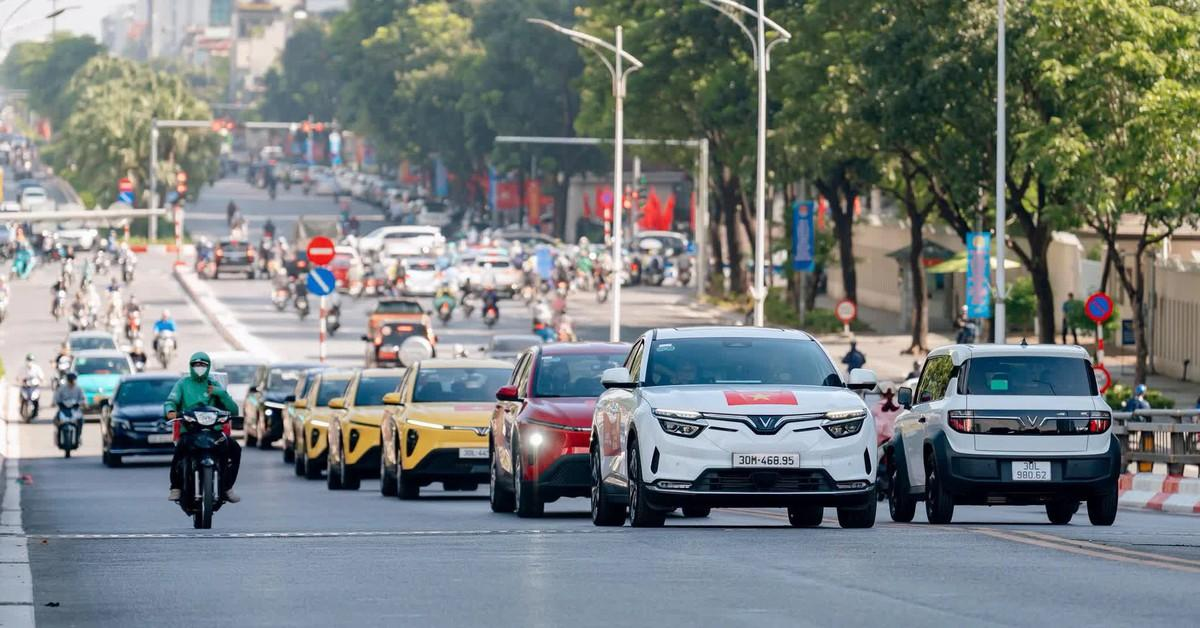
\includegraphics[width=\linewidth,height=4.2cm,keepaspectratio]{nurec-carla/real-driving-data.jpg}\\[3pt]
    \small Dữ liệu thực: camera ghi lại đường, xe và môi trường xung quanh (ảnh minh họa: Tuổi Trẻ Online)
  \end{minipage}\hfill
  \begin{minipage}[t]{0.48\linewidth}
    \centering
    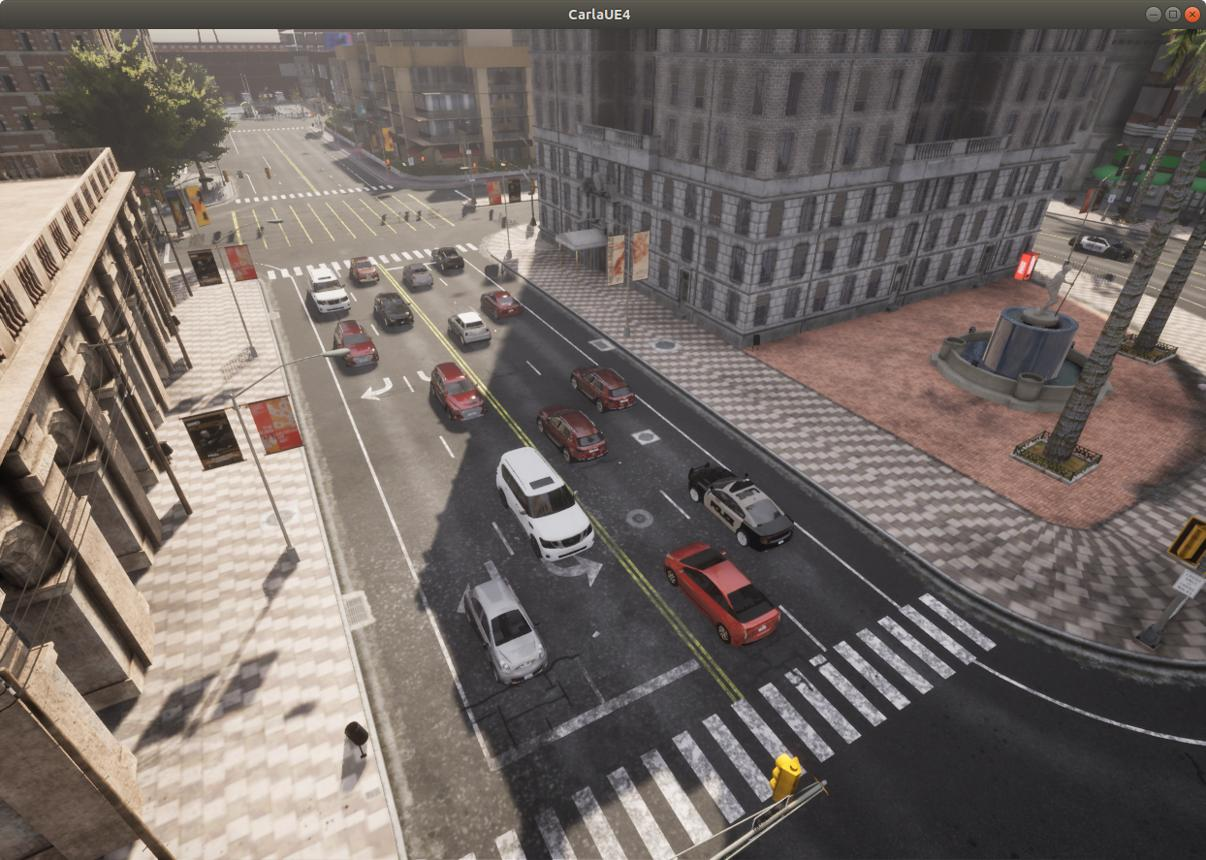
\includegraphics[width=\linewidth,height=4.2cm,keepaspectratio]{nurec-carla/carla-world.jpg}\\[3pt]
    \small Môi trường CARLA: xe và giao thông được quản lý trong thế giới ảo (ảnh: tài liệu CARLA)
  \end{minipage}
  \caption{Dữ liệu thực và môi trường CARLA}
\end{figure}

Ví dụ một bài kiểm thử:
\begin{enumerate}
  \item Xe tự lái chạy lại trên đoạn đường đã ghi hình.
  \item Một chiếc xe khác bất ngờ chuyển làn.
  \item Xe tự lái phải phát hiện nguy hiểm và phanh.
  \item Nhóm đổi tốc độ của xe cắt ngang và chạy lại bài kiểm thử.
  \item Hệ thống ghi nhận ADAS có phanh đúng lúc hay không.
\end{enumerate}

Nếu chỉ dùng video gốc thì không thể đổi vị trí camera hay tạo diễn biến mới.
Nếu chỉ dùng CARLA thì mô phỏng được giao thông, nhưng môi trường 3D không nhất thiết giống địa điểm thực.
Kết hợp hai bên cho phép có cả hình ảnh của nơi thật lẫn khả năng tương tác.

\subsection{NuRec làm những việc gì?}

NuRec có 2 công việc cần phân biệt rõ.

\textbf{Công việc A: Reconstruction (tái dựng).}
Đầu vào thường gồm camera, LiDAR, thông số hiệu chuẩn, vị trí xe theo thời gian và nhãn của vật thể chuyển động.
NuRec cần học được: mặt đường, tòa nhà, cây cối nằm ở đâu; môi trường trông thế nào từ nhiều góc; vật thể nào chuyển động; camera và vật thể ở đâu tại mỗi thời điểm.
Kết quả được đóng gói thành một USDZ scene, gồm mô tả scene, model đã train và các trajectory (quỹ đạo của đối tượng theo thời gian).

\begin{figure}[H]
  \centering
  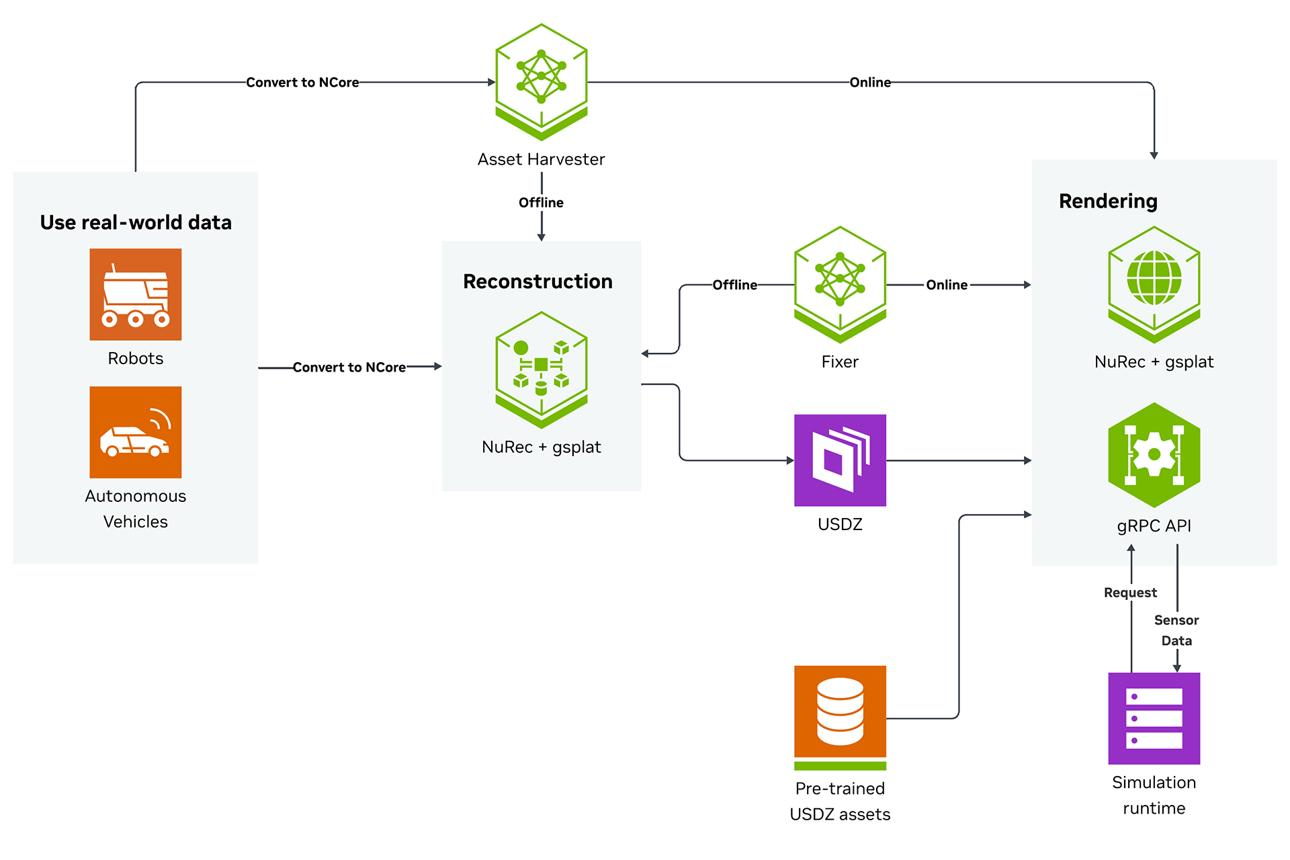
\includegraphics[width=0.85\linewidth]{nurec-carla/nurec-workflow.jpg}
  \caption{Luồng làm việc của NuRec (ảnh: NVIDIA Developer)}
\end{figure}

\textbf{Công việc B: Neural rendering (tạo ảnh).}
Đây là phần quan trọng khi kết hợp với CARLA.
Sau khi có scene, chương trình yêu cầu: quan sát cảnh này từ camera tại vị trí $(x, y, z)$, quay theo hướng $R$, ở thời điểm $t$.
NuRec tạo được ảnh từ góc nhìn đó, dù không có video thật quay đúng vị trí ấy. Kỹ thuật này gọi là novel view synthesis.

Ví dụ, xe ngoài đời chạy giữa làn, trong mô phỏng xe dịch sang trái 1 mét, NuRec có thể tạo góc nhìn mới tương ứng.
Khi camera đi quá xa vùng đã ghi nhận, các chi tiết có thể bị méo hoặc thiếu.

\subsection{Kiến trúc 3 thành phần}

Hệ thống gồm 3 thành phần chạy riêng biệt.
CARLA Server không tự gửi dữ liệu sang NuRec: Python script là phần gọi cả hai bên.

\begin{figure}[H]
  \centering
  \begin{tikzpicture}[
      box/.style={draw=accent, fill=blue!4, rounded corners=2pt, align=center,
                  text width=3.9cm, minimum height=2.5cm, font=\scriptsize\sffamily},
      result/.style={draw=accent, fill=blue!4, rounded corners=2pt, align=center,
                  text width=6cm, minimum height=0.8cm, font=\scriptsize\sffamily},
      flow/.style={<->, >={Stealth[length=2mm]}, thick, color=black!65},
      one/.style={-{Stealth[length=2mm]}, thick, color=black!65},
      lbl/.style={font=\tiny\sffamily, color=black!70}]
    \node[box] (carla) at (-5.4,0) {\textbf{CARLA Server}\\[2pt]Road map, world\\Ego vehicle\\Các xe khác\\Vật lý, thời gian mô phỏng};
    \node[box] (py) at (0,0) {\textbf{Python script}\\[2pt]Điều phối mô phỏng\\Gọi cả hai API\\Đồng bộ camera và thời gian};
    \node[box] (nr) at (5.4,0) {\textbf{NuRec Container}\\[2pt]Reconstructed scene\\Neural renderer\\Camera model};
    \node[result] (img) at (0,-2.3) {\textbf{Dữ liệu cảm biến mô phỏng}: ảnh camera do NuRec tạo};
    \draw[flow] (carla) -- node[lbl, above] {CARLA API} (py);
    \draw[flow] (py) -- node[lbl, above] {gRPC API} (nr);
    \draw[one] (py) -- (img);
  \end{tikzpicture}
  \caption{Kiến trúc NuRec + CARLA}
\end{figure}

\textbf{API} là giao diện để một chương trình yêu cầu chương trình khác làm việc.
Ví dụ, qua CARLA API, script lấy được trạng thái thế giới và vị trí xe:

\begin{lstlisting}[language=Python, numbers=none, caption={Đọc trạng thái qua CARLA API}]
world = client.get_world()
vehicle_pose = vehicle.get_transform()
\end{lstlisting}

\textbf{gRPC} là công nghệ gọi hàm từ xa giữa các chương trình.
Script gửi yêu cầu render đến NuRec Container và nhận lại ảnh.
Dưới đây là yêu cầu thật, rút gọn từ hàm \texttt{generate\_request} trong \texttt{nurec\_integration.py}:

\begin{lstlisting}[language=Python, numbers=none, texcl=true, caption={Yêu cầu render gửi đến NuRec (rút gọn từ mã nguồn CARLA)}]
RGBRenderRequest(
    scene_id=scene_id,
    resolution_h=int(camera_spec.resolution_h * scale),
    resolution_w=int(camera_spec.resolution_w * scale),
    camera_intrinsics=camera_spec,
    frame_start_us=timestamp,
    frame_end_us=timestamp + 1,      # hai giá trị phải khác nhau
    sensor_pose=PosePair(start_pose=pose, end_pose=pose),
    dynamic_objects=dynamic_objects, # vị trí các xe lấy từ CARLA
    image_format=ImageFormat.JPEG,
    image_quality=95,
)
\end{lstlisting}

Trong đó:
\begin{itemize}
  \item \texttt{scene\_id}: scene được chọn.
  \item \texttt{camera\_intrinsics}: thông số bên trong camera như tiêu cự, điểm chính và mô hình biến dạng.
  \item \texttt{sensor\_pose}: vị trí và hướng camera trong thế giới 3D.
  \item \texttt{frame\_start\_us}, \texttt{frame\_end\_us}: thời điểm cần render, tính bằng micro giây.
  \item \texttt{dynamic\_objects}: các vật thể chuyển động và vị trí của chúng.
\end{itemize}

\subsection{Một vòng mô phỏng}

Một vòng closed-loop đầy đủ diễn ra như sau. Thuật toán ADAS ở bước 4 không có sẵn trong ví dụ của CARLA, nhóm phải tự nối vào.

\begin{figure}[H]
  \centering
  \begin{tikzpicture}[
      box/.style={draw=accent, fill=blue!4, rounded corners=2pt, align=center,
                  text width=2.45cm, minimum height=1.25cm, font=\scriptsize\sffamily},
      flow/.style={-{Stealth[length=2mm]}, thick, color=black!65},
      lbl/.style={font=\tiny\sffamily, color=black!70}]
    \node[box] (a) at (0,0) {\textbf{1. CARLA}\\Cập nhật vị trí xe và đồng hồ};
    \node[box] (b) at (3.2,0) {\textbf{2. Python}\\Đọc vị trí camera và thời điểm};
    \node[box] (c) at (6.4,0) {\textbf{3. NuRec}\\Render ảnh camera};
    \node[box] (d) at (9.6,0) {\textbf{4. ADAS}\\Phát hiện, lên đường đi, ra lệnh};
    \node[box] (e) at (12.8,0) {\textbf{5. CARLA}\\Nhận lệnh ga, phanh, lái};
    \draw[flow] (a) -- (b);
    \draw[flow] (b) -- (c);
    \draw[flow] (c) -- (d);
    \draw[flow] (d) -- (e);
    \draw[flow] (e.south) -- ++(0,-0.5) -| node[lbl, pos=0.25, below] {bước mô phỏng tiếp theo} (a.south);
  \end{tikzpicture}
  \caption{Một vòng closed-loop}
\end{figure}

\subsection{Ví dụ của CARLA thực sự làm gì?}

File ví dụ tên là \texttt{example\_nurec\_replay\_save\_images.py}, và tài liệu CARLA gọi đây là replay.
Tuy nhiên, đọc mã nguồn cho thấy ví dụ này đã làm nhiều hơn replay thuần túy:

\begin{itemize}
  \item Ban đầu, xe ego được đặt lại theo quỹ đạo đã ghi bằng \texttt{set\_transform}, chưa bật vật lý.
  \item Sau 1 giây, script gọi \texttt{set\_ego\_simple\_trajectory\_following()}. Xe ego được bật vật lý và do bộ điều khiển \texttt{SimpleTrajectoryFollower} lái bằng lệnh ga, phanh, lái.
  \item Vị trí camera gửi cho NuRec được tính từ vị trí hiện tại của xe trong CARLA (\texttt{actor.get\_transform()}), không phải từ quỹ đạo đã ghi.
  \item Mã nguồn có sẵn \texttt{apply\_ego\_control(control)} để đưa lệnh lái từ bên ngoài vào xe.
\end{itemize}

Như vậy, phần ảnh đã đi theo xe trong CARLA. Phần còn thiếu là bộ điều khiển trong ví dụ chỉ bám theo quỹ đạo đã ghi và không dùng ảnh camera.
Muốn có closed-loop đúng nghĩa, cần thay bộ điều khiển đó bằng thuật toán nhận ảnh từ NuRec.

\begin{table}[H]
  \centering
  \caption{Replay, ví dụ của CARLA và closed-loop}
  \begin{tabularx}{\linewidth}{>{\raggedright\arraybackslash}p{2.9cm} X X X}
    \toprule
     & \textbf{Replay thuần} & \textbf{Ví dụ của CARLA} & \textbf{Closed-loop} \\
    \midrule
    Xe ego & Theo quỹ đạo ghi sẵn & Bám quỹ đạo ghi sẵn, có vật lý & Theo lệnh của ADAS \\
    \addlinespace
    Ảnh & Render theo vị trí replay & Render theo vị trí xe trong CARLA & Render theo vị trí xe trong CARLA \\
    \addlinespace
    Lệnh lái lấy từ & Không có & Bộ bám quỹ đạo & ADAS dựa trên ảnh \\
    \addlinespace
    Quyết định ảnh hưởng đến cảnh sau & Không & Có, nhưng không dựa trên ảnh & Có \\
    \bottomrule
  \end{tabularx}
\end{table}

\begin{warning}
Chạy được script replay không chứng minh đã có closed-loop ADAS.
Vẫn cần nối AD Stack và kiểm tra lệnh điều khiển thực sự tác động vào trạng thái CARLA.
\end{warning}

\subsection{NuRec có tự tạo road logic cho CARLA không?}

Không nên mặc định là có.
Một scene có thể chứa hình ảnh vạch kẻ làn và đèn giao thông rất thật, nhưng simulator chưa chắc hiểu được các thông tin đó.

\begin{table}[H]
  \centering
  \caption{Hình ảnh tái dựng khác với road logic}
  \begin{tabularx}{\linewidth}{>{\raggedright\arraybackslash}p{3cm} X X}
    \toprule
    \textbf{Thành phần} & \textbf{NuRec reconstruction} & \textbf{Road logic / CARLA} \\
    \midrule
    Vạch kẻ đường & Có thể tái dựng & Cần biết ranh giới và kết nối làn \\
    \addlinespace
    Đèn đỏ & Có thể render & Cần trạng thái và quy tắc điều khiển \\
    \addlinespace
    Mặt đường & Có lớp road geometry & Cần mặt đường lái được, hình học và vật lý phù hợp \\
    \addlinespace
    Xe đang chạy & Có thể tái dựng và chỉnh track & Cần hành vi và quỹ đạo đồng bộ với simulator \\
    \addlinespace
    Ngã tư & Có thể tái dựng cảnh & Cần kết nối làn và quy tắc ưu tiên \\
    \bottomrule
  \end{tabularx}
\end{table}

Tài liệu NVIDIA cho biết USDZ có thể chứa bản đồ OpenDRIVE nhưng không bắt buộc.
Tuy nhiên, script của CARLA đọc \texttt{map.xodr} từ USDZ và báo lỗi nếu không có.
CARLA dùng file này để tạo thế giới bằng \texttt{generate\_opendrive\_world}.
Vì vậy, muốn đi theo cách này, scene của nhóm phải có bản đồ OpenDRIVE khớp với cảnh tái dựng.

Ngoài ra, đổi vị trí hiển thị của một xe trong NuRec chưa có nghĩa xe đó có hành vi lái, logic tránh va chạm và trạng thái vật lý trong CARLA.

\subsection{Liên hệ với kiến trúc của nhóm}

Cách làm này khớp với 2 giai đoạn ở chương 2.
Giai đoạn offline chạy trước và thường tốn tính toán hơn. Giai đoạn online lặp lại ở từng bước mô phỏng.

\begin{figure}[H]
  \centering
  \begin{tikzpicture}[
      box/.style={draw=accent, fill=blue!4, rounded corners=2pt, align=center,
                  text width=2.6cm, minimum height=1cm, font=\scriptsize\sffamily},
      flow/.style={-{Stealth[length=2mm]}, thick, color=black!65},
      lbl/.style={font=\tiny\sffamily, color=black!70},
      stage/.style={font=\scriptsize\sffamily\bfseries, color=accent, anchor=west}]
    \node[stage] at (-1.4,1) {Offline: tái dựng};
    \node[box] (a) at (0,0) {Dữ liệu thật};
    \node[box] (b) at (3.6,0) {Chuẩn bị dữ liệu\\camera, LiDAR, pose, track};
    \node[box] (c) at (7.2,0) {NuRec reconstruction};
    \node[box] (d) at (10.8,0) {USDZ scene};
    \node[stage] at (-1.4,-1.1) {Online: mô phỏng};
    \node[box] (e) at (10.8,-2.1) {NuRec renderer};
    \node[box] (f) at (7.2,-2.1) {Ảnh tổng hợp};
    \node[box] (g) at (3.6,-2.1) {AD Stack};
    \node[box] (h) at (0,-2.1) {CARLA World};
    \draw[flow] (a) -- (b);
    \draw[flow] (b) -- (c);
    \draw[flow] (c) -- (d);
    \draw[flow] (d) -- (e);
    \draw[flow] (e) -- (f);
    \draw[flow] (f) -- (g);
    \draw[flow] (g) -- node[lbl, above] {lệnh lái} (h);
    \draw[flow] (h.south) -- ++(0,-0.5) -| node[lbl, pos=0.25, below] {vị trí camera và thời điểm} (e.south);
  \end{tikzpicture}
  \caption{Offline và online trong NuRec + CARLA}
\end{figure}

Song song, cần chuẩn bị bản đồ và road logic để CARLA điều khiển xe đúng với địa điểm thật.
Việc đồng bộ giữa cảnh, bản đồ, xe và ảnh cảm biến quyết định hệ thống có dùng được cho ADAS testing hay không.

Để đánh giá NuRec làm baseline, cần tách 3 câu hỏi:
\begin{enumerate}
  \item \textbf{Reconstruction:} NuRec dựng cảnh chính xác, nhanh và tiết kiệm đến đâu?
  \item \textbf{Integration:} làm sao đồng bộ scene với bản đồ, các xe và camera trong CARLA?
  \item \textbf{Closed-loop:} khi ADAS đổi hành động của xe, ảnh và trạng thái thế giới có cập nhật nhất quán không?
\end{enumerate}

\section{Bản phân tích để tự triển khai}

Mục này tách cách nối của CARLA thành từng phần để nhóm làm lại cho method khác.
Bảng dưới được đọc từ mã nguồn trong thư mục \texttt{PythonAPI/examples/nvidia/nurec}.

\begin{table}[H]
  \centering
  \small
  \caption{Các phần cần có của bộ nối, theo mã nguồn CARLA}
  \begin{tabularx}{\linewidth}{>{\raggedright\arraybackslash}p{2.7cm} >{\raggedright\arraybackslash}X >{\raggedright\arraybackslash}X}
    \toprule
    \textbf{Phần} & \textbf{CARLA làm thế nào} & \textbf{Nhóm cần gì} \\
    \midrule
    Khởi động renderer & \texttt{NuRecRenderService} chạy NuRec trong Docker, mặc định cổng 46435 & Chạy renderer của method thành một service riêng \\
    \addlinespace
    Tạo thế giới & Đọc \texttt{map.xodr} trong USDZ, gọi \texttt{generate\_opendrive\_world} & File OpenDRIVE khớp với cảnh \\
    \addlinespace
    Khớp tọa độ & Ma trận \texttt{t\_scenario\_carla} chuyển giữa scene và CARLA & Tính phép biến đổi tọa độ, kiểm tra bằng ảnh \\
    \addlinespace
    Đồng hồ & Synchronous mode, \texttt{fixed\_delta\_seconds} bằng 1/60 giây & Cố định bước thời gian để render khớp mô phỏng \\
    \addlinespace
    Xe khác & Tạo actor CARLA từ track trong USDZ, di chuyển bằng \texttt{set\_transform} & Track của vật thể động, kích thước xe \\
    \addlinespace
    Render theo tick & \texttt{world.on\_tick} gọi render; \texttt{NurecSensor} tính vị trí camera từ actor & Callback ở mỗi tick, giới hạn tốc độ render \\
    \addlinespace
    Gửi vật thể động & \texttt{generate\_request} đổi vị trí actor sang \texttt{DynamicObject} & Renderer phải nhận được vị trí vật thể theo từng khung hình \\
    \addlinespace
    Nhận lệnh lái & \texttt{apply\_ego\_control}, \texttt{set\_ego\_autopilot} & Nối AD Stack vào điểm này \\
    \bottomrule
  \end{tabularx}
\end{table}

Vòng lặp closed-loop có thể viết theo khung sau. Đây là mã minh họa, chưa chạy thử; tên \texttt{ad\_stack} là giả định.

\begin{lstlisting}[language=Python, texcl=true, caption={Khung closed-loop dựa trên NurecScenario (minh họa)}]
latest = {}

def on_image(image):              # NuRec gọi hàm này khi có ảnh mới
    latest["front"] = image

with NurecScenario(client, usdz_path, port=46435, fps=30) as scenario:
    scenario.add_camera(camera_name, on_image, framerate=10)
    scenario.start_replay()
    while not scenario.is_done():
        scenario.tick()               # CARLA chạy một bước, NuRec render
        if "front" in latest:
            control = ad_stack.step(latest["front"])   # ảnh sang lệnh lái
            scenario.apply_ego_control(control)      # lệnh vào xe trong CARLA
\end{lstlisting}

Các điểm cần kiểm tra trước khi làm theo:
\begin{itemize}
  \item \textbf{Chỉ có camera:} mã nguồn CARLA không gọi \texttt{render\_lidar}. Muốn có LiDAR từ NuRec thì phải tự thêm.
  \item \textbf{Xe rời xa đường đã ghi:} ảnh có thể bị méo, cần đo khi xe lệch khỏi quỹ đạo.
  \item \textbf{Xe khác chưa phản ứng:} các xe mặc định chạy theo track đã ghi, không tự tránh ego. Có thể chuyển sang Traffic Manager, nhưng mã nguồn hiện đặt các xe này bỏ qua đèn và xe khác.
  \item \textbf{Khớp hai thế giới:} bề mặt va chạm trong CARLA tạo từ OpenDRIVE, có thể lệch so với cảnh NuRec.
  \item \textbf{Phiên bản API:} tài liệu NuRec 26.03 ghi cần \texttt{--enable-editing-actors} để đổi vị trí actor, còn lệnh khởi động trong CARLA không có cờ này. Bản mới dùng \texttt{render\_camera} thay cho \texttt{render\_rgb}. Cần kiểm tra theo phiên bản container.
  \item \textbf{Tốc độ:} renderer phải đủ nhanh, vì trong synchronous mode mô phỏng chờ từng bước.
\end{itemize}

Muốn nối một method khác, ví dụ 3DGS tự train, nhóm cần viết 3 phần: service render nhận vị trí camera và trả ảnh, phép biến đổi tọa độ sang CARLA, và file OpenDRIVE cho khu vực đó.

\section{Road logic}

Hướng làm: thử lần lượt manual baseline, bản đồ có sẵn và trích xuất tự động.

\section{Geometry}

Hướng làm: kiểm tra khả năng tạo bề mặt và đưa vào mô phỏng.

\section{Traffic simulation}

Hướng làm: chạy các phương tiện khác trong CARLA và kiểm tra tương tác với ego vehicle.

\section{Baseline CARLA}

Hướng làm: chạy CARLA với bản đồ có sẵn, xác định đầu vào cần cho một khu vực mới.


% ---------- Part III: cả nhóm tổng hợp ----------
\part{Synthesis, Selection \& Integration}
\chapter{Comparative Evaluation (So sánh các approach)}

\section{Tổng hợp kết quả}

Hướng làm: gom kết quả của 4 approach về cùng một bảng theo protocol ở chương 4.

\section{So sánh theo track}

Hướng làm: so sánh pinhole và fisheye, nêu nguyên nhân khác biệt.

\section{So sánh theo tiêu chí}

Hướng làm: so sánh theo cost, quality, robustness và compatibility.

\section{Kết luận so sánh}

Hướng làm: nêu approach phù hợp với từng track, kèm bằng chứng.

\chapter{Final Pipeline Design (Thiết kế pipeline cuối)}

Pipeline tổng hợp không còn là pipeline gốc của một paper, nên cần thiết kế và kiểm chứng riêng.
Hybrid pipeline là phần mở rộng. Nếu không tốt hơn baseline, nhóm chọn một approach gốc làm reference pipeline.

\section{Lựa chọn pipeline}

Hướng làm: chọn approach tốt nhất hoặc đề xuất hybrid pipeline, nêu lý do chọn từng module.

\section{Sơ đồ pipeline}

Hướng làm: vẽ pipeline cuối và các điểm nối giữa module.

\section{Kiểm chứng}

Hướng làm: chạy thực nghiệm riêng và so sánh với baseline.

\chapter{Framework Implementation \& Validation (Triển khai và kiểm chứng framework)}

\section{Implementation status}

\begin{table}[H]
  \centering
  \caption{Tình trạng module}
  \begin{tabularx}{\linewidth}{X l l l}
    \toprule
    \textbf{Module} & \textbf{Đã thiết kế} & \textbf{Đã triển khai} & \textbf{Đã kiểm chứng} \\
    \midrule
     &  &  &  \\
    \bottomrule
  \end{tabularx}
\end{table}

\section{Tích hợp các approach vào tool}

Hướng làm: đưa các approach vào tool qua adapter, so kết quả với số liệu ở Part II để phát hiện sai lệch.

\section{Module swapping}

Hướng làm: kiểm tra đổi được method và thứ tự module theo từng approach.

\section{Experiment management}

Hướng làm: kiểm tra việc cấu hình, ghi log và tổng hợp kết quả thí nghiệm.

\section{Reproducibility và determinism}

Hướng làm: chạy lại cùng cấu hình và đo mức nhất quán.

\chapter{CARLA Integration Feasibility (Khả năng tích hợp CARLA)}

\section{Simulation interface}

Hướng làm: thử nối scene, road logic và traffic vào CARLA.

\section{Neural renderer}

Hướng làm: kiểm tra từng method có nối được với CARLA không và cần những gì.

\section{Geometry và road logic gaps}

Hướng làm: ghi các phần còn thiếu so với yêu cầu, dựa trên chương Supporting Study.

\section{AD Stack và closed-loop}

Hướng làm: xác định mức đạt được, từ controller đơn giản đến các AD module có sẵn.

\section{Feasibility matrix}

Hướng làm: tổng hợp từng method theo khả năng tích hợp với CARLA, road logic, geometry và renderer.

\chapter{Conclusions \& Future Work (Kết luận và hướng phát triển)}

\section{Kết quả cuối cùng}

Hướng làm: đối chiếu kết quả với yêu cầu ở chương 1.

\section{Đã và chưa kiểm chứng}

Hướng làm: nêu rõ phần đã thiết kế, đã triển khai và đã kiểm chứng.

\section{Technical limitations}

Hướng làm: ghi lại các giới hạn đã gặp, kèm bằng chứng.

\section{Hướng phát triển}

Hướng làm: ghi các phần còn lại của M3--M5 và điều kiện để tiếp tục.


% ---------- Khái niệm ----------
\chapter{Tổng hợp khái niệm}

\section{ADAS và các cấp độ L1, L2, L2+}

ADAS (Advanced Driver Assistance Systems) là hệ thống hỗ trợ người lái, chẳng hạn giữ làn, điều khiển tốc độ và phanh khẩn cấp.

\begin{table}[H]
  \centering
  \caption{Các cấp độ hỗ trợ lái}
  \begin{tabularx}{\linewidth}{l X}
    \toprule
    \textbf{Cấp độ} & \textbf{Khả năng} \\
    \midrule
    L1 & Hỗ trợ điều khiển ngang hoặc dọc \\
    L2 & Hỗ trợ đồng thời điều khiển ngang (đánh lái) và dọc (tăng/giảm tốc), nhưng người lái vẫn phải giám sát \\
    L2+ & Thuật ngữ thương mại/kỹ thuật cho các hệ thống L2 tiên tiến, có thể hỗ trợ thêm điều hướng hoặc chuyển làn trong điều kiện cho phép \\
    \bottomrule
  \end{tabularx}
\end{table}

L2+ không phải cấp độ tự động hóa chính thức của SAE.
Về trách nhiệm giám sát, hệ thống L2+ vẫn thuộc L2.

\section{L2/L2+ ADAS Resimulation}

Resimulation là quá trình chạy lại hoặc tái tạo các tình huống lái xe để kiểm thử, đánh giá và cải tiến hệ thống ADAS, mà không cần đưa xe ra đường thực tế mỗi lần thử nghiệm.

Resimulation không đơn thuần là phát lại video hoặc tái dựng môi trường 3D.
Resimulation phải cho phép kiểm tra hệ thống ADAS sẽ nhận biết, quyết định và phản ứng như thế nào trong một tình huống lái xe.

Dữ liệu thường được thu từ xe chạy ngoài đường:
\begin{itemize}
  \item Camera ghi lại hình ảnh giao thông.
  \item LiDAR/Radar đo các đối tượng xung quanh (nếu có).
  \item GPS/IMU ghi nhận chuyển động và vị trí xe.
  \item CAN bus ghi tốc độ, góc lái, trạng thái phanh và các tín hiệu khác.
\end{itemize}

Sau đó, kỹ sư dùng dữ liệu này để chạy lại tình huống và kiểm thử phiên bản mới của thuật toán ADAS:

\begin{figure}[H]
  \centering
  \begin{tikzpicture}[
      box/.style={draw=accent, fill=blue!4, rounded corners=2pt, align=center,
                  minimum width=3.3cm, text width=3.1cm, minimum height=1.3cm,
                  font=\scriptsize\sffamily},
      flow/.style={-{Stealth[length=2mm]}, thick, color=black!65}]
    \node[box] (a) at (0,0) {\textbf{Real-world driving logs}\\Camera, LiDAR, GPS/IMU, CAN};
    \node[box] (b) at (3.95,0) {\textbf{Resimulation environment}\\Dữ liệu phát lại hoặc môi trường tái dựng};
    \node[box] (c) at (7.9,0) {\textbf{ADAS software stack}\\Perception, prediction, planning, control};
    \node[box] (d) at (11.85,0) {\textbf{Evaluation \& regression testing}\\Va chạm, lệch làn, phanh, quỹ đạo, độ êm};
    \draw[flow] (a) -- (b);
    \draw[flow] (b) -- (c);
    \draw[flow] (c) -- (d);
  \end{tikzpicture}
  \caption{Pipeline khái niệm của resimulation}
\end{figure}

Ví dụ: xe đang chạy 60~km/h thì một ô tô phía trước bất ngờ chuyển làn.
Resimulation giúp kiểm tra thuật toán ADAS có phát hiện xe chuyển làn, dự đoán nguy cơ va chạm và ra lệnh phanh phù hợp hay không.

\section{Open-loop và closed-loop}

Khác biệt nằm ở chỗ quyết định của thuật toán có làm thay đổi dữ liệu đầu vào tiếp theo hay không.

\begin{table}[H]
  \centering
  \caption{So sánh open-loop và closed-loop}
  \begin{tabularx}{\linewidth}{>{\raggedright\arraybackslash}p{2.6cm} X X}
    \toprule
     & \textbf{Open-loop} & \textbf{Closed-loop} \\
    \midrule
    Cách hoạt động & Chạy lại thuật toán trên dữ liệu cảm biến đã ghi sẵn & Simulator cập nhật môi trường theo trạng thái xe, rồi sinh dữ liệu cảm biến mới \\
    \addlinespace
    Tác động của quyết định lái & Không làm thay đổi dữ liệu đầu vào tiếp theo & Làm thay đổi trạng thái xe và dữ liệu đầu vào tiếp theo \\
    \addlinespace
    Phù hợp để kiểm thử & Perception, prediction, phát hiện regression (lỗi phát sinh sau khi cập nhật phần mềm) & Toàn bộ chu trình perception $\to$ planning $\to$ control và hậu quả của quyết định lái \\
    \bottomrule
  \end{tabularx}
\end{table}

Trong công nghiệp, resimulation thường mang nghĩa open-loop replay/recompute\footnote{Nguồn gốc trong trao đổi: ISE Developer Blog, \url{https://devblogs.microsoft.com}}.
Closed-loop resimulation là dạng mở rộng, khi tình huống thực tế được tái tạo thành môi trường có thể tương tác.

\section{Simulation và resimulation}

\begin{table}[H]
  \centering
  \caption{So sánh simulation và resimulation}
  \begin{tabularx}{\linewidth}{>{\raggedright\arraybackslash}p{3cm} X X}
    \toprule
     & \textbf{Simulation} & \textbf{Resimulation} \\
    \midrule
    Nguồn tình huống & Có thể tạo hoàn toàn nhân tạo & Thường bắt đầu từ dữ liệu hoặc tình huống đã ghi nhận \\
    \addlinespace
    Mục tiêu & Kiểm thử tình huống giả định & Tái hiện, phân tích hoặc kiểm thử lại tình huống cụ thể \\
    \addlinespace
    Ví dụ & Tạo giao lộ và cho 10 xe chạy & Tái hiện một tình huống xe thật suýt va chạm \\
    \addlinespace
    Closed-loop & Có & Có, nếu hệ thống hỗ trợ tương tác \\
    \bottomrule
  \end{tabularx}
\end{table}

\section{Liên hệ với project}

Một pipeline khả thi khi áp dụng vào CARLA, NuRec và 3DGS:

\begin{figure}[H]
  \centering
  \begin{tikzpicture}[
      box/.style={draw=accent, fill=blue!4, rounded corners=2pt, align=center,
                  minimum width=2.7cm, text width=2.5cm, minimum height=1.5cm,
                  font=\scriptsize\sffamily},
      flow/.style={-{Stealth[length=2mm]}, thick, color=black!65},
      lbl/.style={font=\tiny\sffamily, color=black!70}]
    \node[box] (a) at (0,0) {\textbf{Dữ liệu thực tế}\\Camera, LiDAR, calibration, vehicle poses};
    \node[box] (b) at (3.3,0) {\textbf{3D reconstruction}\\NuRec/3DGS, render góc nhìn mới};
    \node[box] (c) at (6.6,0) {\textbf{CARLA}\\Road logic, traffic actors, vehicle dynamics};
    \node[box] (d) at (9.9,0) {\textbf{ADAS L2/L2+}\\Nhận sensor data, ra quyết định, điều khiển xe};
    \node[box] (e) at (13.2,0) {\textbf{Evaluation}\\An toàn, quỹ đạo, giữ làn, va chạm, tái lập};
    \draw[flow] (a) -- (b);
    \draw[flow] (b) -- (c);
    \draw[flow] (c) -- (d);
    \draw[flow] (d) -- (e);
    \draw[flow] (d.south) -- ++(0,-0.5) -| node[lbl, pos=0.25, below] {closed-loop feedback} (c.south);
  \end{tikzpicture}
  \caption{Pipeline khả thi của project}
\end{figure}

\begin{itemize}
  \item \textbf{NuRec/3DGS:} tạo nền hình ảnh gần với khu vực đường thật và render ảnh từ vị trí camera mới.
  \item \textbf{Road logic layer:} mô tả làn đường, kết nối làn, giao lộ và quy tắc giao thông để xe lập kế hoạch di chuyển.
  \item \textbf{CARLA:} mô phỏng xe, traffic actors, thời gian và tương tác.
  \item \textbf{ADAS stack:} hệ thống cần được kiểm thử.
\end{itemize}

\begin{warning}
Có NuRec và CARLA không tự động bảo đảm closed-loop hoạt động.
Vẫn cần tích hợp tọa độ, road logic, sensor rendering và vòng điều khiển xe.
\end{warning}

\begin{keyidea}[Kết luận]
Với mục tiêu mentor đã mô tả (closed-loop trên khu vực địa lý có thật, chi phí thấp, mở rộng được, tính xác định cao), project đang hướng đến real-world-based closed-loop ADAS simulation/resimulation, không chỉ là công cụ replay camera hay tái dựng 3DGS.

Đầu ra quan trọng nhất không phải một scene 3D đẹp, mà là một môi trường kiểm thử nơi hệ thống L2/L2+ chạy, tương tác và được đánh giá có thể tái lập.
\end{keyidea}


% =====================================================================
\bibliographystyle{plainnat}
\bibliography{references}

\end{document}
